%% Verze pro jednostranný tisk:
%\documentclass[11pt,a4paper]{report}
%\usepackage[top=25mm,bottom=25mm,right=25mm,left=30mm,head=12.5mm,foot=12.5mm]{geometry}
%\let\openright=\clearpage

%% Pokud tiskneme oboustranně:
\documentclass[11pt,a4paper,twoside,openright]{report}
\usepackage[top=25mm,bottom=25mm,right=25mm,left=30mm,head=12.5mm,foot=12.5mm]{geometry}
\let\openright=\cleardoublepage

%% Definice různých užitečných maker (viz popis uvnitř souboru)
%%% Tento soubor obsahuje definice různých užitečných maker a prostředí %%%
%%% Další makra připisujte sem, ať nepřekáží v ostatních souborech.     %%%

\usepackage[a-2u]{pdfx}     % výsledné PDF bude ve standardu PDF/A-2u

%%% Nastavení pro použití samostatné bibliografické databáze.
\usepackage[
   backend=bibtex
  ,style=iso-authoryear
  %,style=iso-numeric
  ,sortlocale=cs_CZ
  ,bibencoding=UTF8
  %,block=ragged
]{biblatex}
\let\cite\parencite
\bibliography{literatura}

%% Přepneme na českou sazbu, fonty Latin Modern a kódování češtiny
\usepackage[czech]{babel}
\usepackage{lmodern}
\usepackage[T1]{fontenc}
\usepackage{textcomp}
\usepackage[utf8]{inputenc}
\usepackage{float}

%%% Další užitečné balíčky (jsou součástí běžných distribucí LaTeXu)
\usepackage{xcolor}
\usepackage{amsmath}        % rozšíření pro sazbu matematiky
\usepackage{amsfonts}       % matematické fonty
\usepackage{amsthm}         % sazba vět, definic apod.
\usepackage{bm}             % tučné symboly (příkaz \bm)
\usepackage{graphicx}       % vkládání obrázků
\usepackage{fancyvrb}       % vylepšené prostředí pro strojové písmo
\usepackage{fancyhdr}       % prostředí pohodlnější nastavení hlavy a paty stránek
\usepackage{icomma}         % inteligetní čárka v matematickém módu
\usepackage{dcolumn}        % lepší zarovnání sloupců v tabulkách
\usepackage{booktabs}       % lepší vodorovné linky v tabulkách
\makeatletter
\@ifpackageloaded{xcolor}{
   \@ifpackagewith{xcolor}{usenames}{}{\PassOptionsToPackage{usenames}{xcolor}}
  }{\usepackage[usenames]{xcolor}} % barevná sazba
\makeatother
\usepackage{multicol}       % práce s více sloupci na stránce
\usepackage{caption}
\usepackage{enumitem}
\setlist[itemize]{noitemsep, topsep=0pt, partopsep=0pt}
\setlist[enumerate]{noitemsep, topsep=0pt, partopsep=0pt}
\setlist[description]{noitemsep, topsep=0pt, partopsep=0pt}

\usepackage{tocloft}
\setlength\cftparskip{0pt}
\setlength\cftbeforechapskip{1.5ex}
\setlength\cftfigindent{0pt}
\setlength\cfttabindent{0pt}
\setlength\cftbeforeloftitleskip{0pt}
\setlength\cftbeforelottitleskip{0pt}
\setlength\cftbeforetoctitleskip{0pt}
\renewcommand{\cftlottitlefont}{\Huge\bfseries\sffamily}
\renewcommand{\cftloftitlefont}{\Huge\bfseries\sffamily}
\renewcommand{\cfttoctitlefont}{\Huge\bfseries\sffamily}

% vyznaceni odstavcu
\parindent=0pt
\parskip=11pt

% zakaz vdov a sirotku - jednoradkovych pocatku ci koncu odstavcu na prechodu mezi strankami
\clubpenalty=10000
\widowpenalty=10000
\displaywidowpenalty=10000
\raggedbottom

% nastaveni radkovani
\renewcommand{\baselinestretch}{1.20}

% nastaveni pro nadpisy - tucne a bezpatkove
\usepackage{sectsty}    
\allsectionsfont{\sffamily}

% nastavení hlavy a paty stránek
\fancyhf{}
\fancyhead[RO,LE]{\rightmark}
\fancyfoot[RO,LE]{\thepage}
\renewcommand{\footrulewidth}{.5pt}
\fancypagestyle{plain}{%
\fancyhf{} % clear all header and footer fields
\fancyfoot[RO,LE]{\thepage}
\renewcommand{\headrulewidth}{0pt}
\renewcommand{\footrulewidth}{0.5pt}}

% Tato makra přesvědčují mírně ošklivým trikem LaTeX, aby hlavičky kapitol
% sázel příčetněji a nevynechával nad nimi spoustu místa. Směle ignorujte.
\makeatletter
\def\@makechapterhead#1{
  {\parindent \z@ \raggedright \sffamily
   \Huge\bfseries \thechapter. #1
   \par\nobreak
   \vskip 20\p@
}}
\def\@makeschapterhead#1{
  {\parindent \z@ \raggedright \sffamily
   \Huge\bfseries #1
   \par\nobreak
   \vskip 20\p@
}}
\makeatother

% Trochu volnější nastavení dělení slov, než je default.
\lefthyphenmin=2
\righthyphenmin=2

% Zapne černé "slimáky" na koncích řádků, které přetekly, abychom si
% jich lépe všimli.
\overfullrule=1mm

%% Balíček hyperref, kterým jdou vyrábět klikací odkazy v PDF,
%% ale hlavně ho používáme k uložení metadat do PDF (včetně obsahu).
%% Většinu nastavítek přednastaví balíček pdfx.
\hypersetup{unicode}
\hypersetup{breaklinks=true}
\hypersetup{hidelinks}

%%% Prostředí pro sazbu kódu, případně vstupu/výstupu počítačových
%%% programů. (Vyžaduje balíček fancyvrb -- fancy verbatim.)

\DefineVerbatimEnvironment{code}{Verbatim}{fontsize=\small, frame=single}

% nastavení 

\usepackage{listings}


\definecolor{codegreen}{rgb}{0,0.6,0}
\definecolor{codegray}{rgb}{0.5,0.5,0.5}
\definecolor{codepurple}{rgb}{0.58,0,0.82}
\definecolor{backcolour}{rgb}{0.95,0.95,0.92}

\lstdefinestyle{mystyle}{
	backgroundcolor=\color{backcolour},   
	commentstyle=\color{codegreen},
	keywordstyle=\color{magenta},
	numberstyle=\tiny\color{codegray},
	stringstyle=\color{codepurple},
	basicstyle=\ttfamily\footnotesize,
	breakatwhitespace=false,         
	breaklines=true,                 
	captionpos=b,                    
	keepspaces=true,                 
	numbers=left,                    
	numbersep=5pt,                  
	showspaces=false,                
	showstringspaces=false,
	showtabs=false,                  
	tabsize=2
}

\lstdefinelanguage{JavaScript}{
	morekeywords=[1]{break, continue, delete, else, for, function, if, in,
		new, return, this, typeof, var, void, while, with, class, extends, default},
	% Literals, primitive types, and reference types.
	morekeywords=[2]{false, null, true, boolean, number, undefined,
		Array, Boolean, Date, Math, Number, String, Object, import, from, export, const},
	% Built-ins.
	morekeywords=[3]{eval, parseInt, parseFloat, escape, unescape, render},
	sensitive,
	morecomment=[s]{/*}{*/},
	morecomment=[l]//,
	morecomment=[s]{/**}{*/}, % JavaDoc style comments
	morestring=[b]',
	morestring=[b]"
}[keywords, comments, strings]

\renewcommand{\lstlistingname}{Procedura}% Listing -> Algorithm
\renewcommand{\lstlistlistingname}{Seznam procedur}% List of Listings -> List of Algorithms

\lstset{style=mystyle}
\usepackage{todonotes}
\usepackage{svg}
\usepackage{tabularx}

%%% Údaje o práci
% Název práce v jazyce práce (přesně podle zadání)
\def\NazevPrace{aaaa}

% Typ práce
\def\TypPrace{BAKALÁŘSKÁ PRÁCE}
%\def\TypPrace{DIPLOMOVÁ PRÁCE}


% Jméno autora
\def\AutorPrace{Karel Douda}

% Rok odevzdání. měsíc (slovně)
\def\DatumOdevzdani{květen 2020}

% Vedoucí práce: Jméno a příjmení s~tituly
\def\Vedouci{Ing. David Král}

% Studijní program a obor
\def\StudijniProgram{Aplikovaná informatika}
\def\StudijniObor{Aplikovaná informatika}

% Text čestného prohlášení pro MUŽE pro bakalářskou prácí
\def\Prohlaseni{Prohlašuji, že jsem bakalářskou práci \textit{\NazevPrace} vypracoval samostatně za použití v práci uvedených pramenů a literatury.}
% Text čestného prohlášení pro MUŽE pro diplomovou prácí
%\def\Prohlaseni{Prohlašuji, že jsem diplomovou práci \textit{\NazevPrace} vypracoval samostatně za použití v práci uvedených pramenů a literatury.}
% Text čestného prohlášení pro ŽENY pro bakalářskou prácí
%\def\Prohlaseni{Prohlašuji, že jsem bakalářskou práci \textit{\NazevPrace} vypracovala samostatně za použití v práci uvedených pramenů a literatury.}
% Text čestného prohlášení pro ŽENY pro diplomovou prácí
%\def\Prohlaseni{Prohlašuji, že jsem diplomovou práci \textit{\NazevPrace} vypracovala samostatně za použití v práci uvedených pramenů a literatury.}

% Nepovinné poděkování (vedoucímu práce, konzultantovi, tomu, kdo
% zapůjčil software, literaturu apod.)
\def\Podekovani{%
Poděkování.
}

% Abstrakt (doporučený rozsah cca 150-250 slov; nejedná se o zadání práce)
\def\Abstrakt{%
Abstrakt.
}
\def\AbstraktEN{%
Abstract.
}

% 3 až 5 klíčových slov (doporučeno)
\def\KlicovaSlova{animal tracking, mobilní aplikace, react native, expo}
\def\KlicovaSlovaEN{animal tracking, mobile app, react native, expo}

%% Titulní strana a různé povinné informační strany
\begin{document}
%%% Titulní strana práce a další povinné informační strany

%%% Titulní strana práce

\pagestyle{empty}
\hypersetup{pageanchor=false}

\begin{center}
\Huge\sffamily
Vysoká škola ekonomická v Praze\\
Fakulta informatiky a statistiky

\vspace{\stretch{1}}


\includegraphics[width=.3\textwidth]{img/logo-FIS}

\vspace{\stretch{2}}

\bfseries\NazevPrace

\vspace{8mm}
\mdseries\TypPrace

\vspace{8mm}
\large
\begin{tabular}{rl}
Studijní program: & \StudijniProgram \\
\noalign{\vspace{2mm}}
Studijní obor: & \StudijniObor \\
\end{tabular}

\vspace{\stretch{8}}

\begin{tabular}{rl}
Autor: & \AutorPrace \\
\noalign{\vspace{2mm}}
Vedoucí práce: & \Vedouci \\
\end{tabular}

\vspace{8mm}
Praha, \DatumOdevzdani
\end{center}


\openright

%%% Strana s čestným prohlášením k bakalářské práci

\hypersetup{pageanchor=true}
\pagestyle{plain}
\cleardoublepage
\vspace*{\fill}
\section*{Prohlášení}
\noindent
\Prohlaseni

\vspace{2cm}
\noindent
V Praze dne DD. měsíc RRRR
\hfill%
\begin{minipage}[t]{.5\textwidth}%
\begin{center}
\dotfill\\
Podpis studenta
\end{center}
\end{minipage}
\vspace{1cm}

%%% Poděkování
\openright
\vspace*{\fill}
\section*{Poděkování}
\noindent
\Podekovani
\vspace{1cm}


%%% Povinná informační strana bakalářské práce
\openright
\section*{Abstrakt}
\noindent
\Abstrakt
\subsection*{Klíčová slova}
\noindent
\KlicovaSlova
\clearpage

\bigskip\bigskip\bigskip
\section*{Abstract}
\noindent
\AbstraktEN
\subsection*{Keywords}
\noindent
\KlicovaSlovaEN

\openright


%%% Strana s automaticky generovaným obsahem bakalářské práce
\setcounter{tocdepth}{2}
\tableofcontents

%%% Obrázky v bakalářské práci
\openright
\listoffigures

%%% Tabulky v bakalářské práci (opět nemusí být nutné uvádět)
\clearpage
\listoftables

%%% Použité zkratky v bakalářské práci (opět nemusí být nutné uvádět)
\chapter*{Seznam použitých zkratek}

\begin{multicols}{2}
\raggedright
\begin{description}
\item [IoT] Internet of Things
\item [GSM] Global System for Mobile Communications
\item [GPS] Global Positioning System
\item [HTTP] HyperText Transfer Protocol
\item[CSS] Cascading Style Sheets
\item [JS] JavaScript
\item [SDK] Software Development Kit
\item [NPM] Node Package Manager
\item [ES] EcmaScript
\item [TS] TypeScript
\item [RN] ReactNative
\item [JSON] JavaScript Object Notation
\end{description}
\end{multicols}



\pagestyle{fancy}
%%% Jednotlivé kapitoly práce jsou pro přehlednost uloženy v samostatných souborech
\chapter*{Úvod}
\addcontentsline{toc}{chapter}{Úvod}

S rozvojem IoT technologí dochází ke stále další a další miniaturizaci autonomních off-the-grid zařízení. Jedním z mnoha oborů, které z tohoto vývoje těží, je zoologie. Obory zoologie zabývající se výzkumem migrací, studiem životních cyklů, ochrany a výzkum vlivu lidské činnosti na zvířata díky tomuto vývoji využívají stále dostupnější trackovací zařízení nasazovaná na zvířata. Nasazená zařízení komunikují především pomocí GSM technologií a sbírají telemetrická data o životních funkcích zvířete, pozici, vzdálenosti k zájmovým bodům a podobně.

% proč bylo téma zvoleno	

Cílem této práce je vytvoření aplikace pro sledování a kontrolu divokých zvířat v terénu, konkrétněji ptáků. Primární funkcí aplikace je zobrazení posledních pozic vybraných zvířat v mapě. O vybraných zvířatech se ukládají metainformace, které mohou sloužit k dodatečné identifikaci v terénu. Pro aplikaci je kritická možnost fungování bez internetového připojení, kterou současné řešení nepodporuje. Současné řešení taktéž není vhodné pro použtí na mobilu z hlediska použitelnosti. Toto téma je řešeno z důvodu absence efektivního řešení tohoto problému.

Zvolený způsob řešení je multiplatformní aplikace vyvíjená v prostředí React Native s možností prací offline. React Native umožňuje vytváření mobilních aplikací pro platformy Android i iOS bez nutnosti psát dvě separátní aplikace. React Native je souborem JS knihoven postavených nad frontendovým frameworkem React od společnosti Facebook. Pro zrychlení vývoje bez nutnosti podbroného testování aplikací na obou platformách byla použita nástavba Expo, která dále abstrahuje od platformně závislého kódu. Zdrojem dat je ornitologická platforma Anitra, která mimo funkce datového uložiště podporuje sdílení dat a udržování metainformací o žvířatech.

Tento dokument se skládá z X kapitol. První kapitola ve zkratce popisuje problémovou oblast, současný stav a základní koncepty nutné pro pochopení zbytku práce související s kontextem ornitologie a telemetrických zařízení pro ornitologii. V druhé kapitole se objasní stávající řešení využívaní k docílení určitých požadavků, které objasní následující kapitoly a důvod, proč existující řešení nejsou vhodná. Samotným vývojovým procesem se tento dokument zabývá od kapitoly Analýza požadavků, ve které se uvedou funkční požadavky na mobilní aplikaci. Kapitola technologie popisuje technologie, které pro řešení tohoto problému šlo využít, jaká byla vybrána a základní informace o jednotlivých částech technologie. Kapitola návrh popíše návrh aplikačních architektury a návrh uživatelského rozhraní. Kapitola implementace popíše proces vytváření samotné aplikace a věnuje se specifickému řešení problémů z předchozí kapitoly. Předposlední kapitolou je testování a nasazení, kde je popsán způsob, jakým byla aplikace testována a publikována. Na závěr je zhodnocení splnění cílů práce a možnost dalšího rozvoje.

% Při vývoji byl použitý vodopádový model softwarového inženýrství.

%%% Fiktivní kapitola s ukázkami sazby

\chapter{Problémová oblast}{\tiny }

Sledování a popis životního cyklu ptáků, vědecká disciplína nazývaná ornitologie, je poměrně starou vědeckou disciplínou s kořeny již ve starověku. Jedním z prvních dochovaných textů zabývajícím se popisu života ptáků je Aristotelova \emph{Historia Animalium} v roce 350 př. n. l \cite{historiaAnimalium}, která podrobně popisovala mimojiné i ptačí migrace. Ornitologie se postupně rozvíjela -- zaváděly se taxonomie ptactva, studovala se ptačí anatomie, ale spousta otázek spojena s chováním ptáků zůstavala nezodpovězena. V roce 1805 se Americký ornitolog John James Audubon údajně snažil prokázat, že se každým rokem na jeho farmu vrací stejný jedinec druhu \emph{Sayornis phoebe} přivázáním stříbrného lanka na nohu \cite{halley2018audubon}. Tímto by nepřímo položil základy pro tzv. kroužkování, pasivní označení jedinců kovovým kroužkem s vyraženým sériovým identifikátorem kroužku. Systém kroužkování zavedl dánský ornitolog a učitel Hans Christian Cornelius Mortensen v roku 1899. Na území České republiky se kroužkování ujalo roku 1910, přibližně rok po rozšíření systému v Anglii a Německu. Dle informací Společnosti spolupracovníků kroužkovací stanice Národního muzea je dnes registrováno 480 spolupracovníků, kteří ročně okroužkují kolem 175 000 ptáků \cite{krouzkovaniPtakuHistorie}.

Kroužkování ptáků slouží k mnoha účelům -- mapování migračních tras (zimoviště, návrat na stejné lokace), populační studie (např. rozšiřování jednotlivých druhů, roční úhyn nebo naopak nárůst), životní cyklus ptactva (např. délka života). Kroužkování je dodnes základem práce ornitologů díky jeho nízké cenové náročnosti a mezinárodní kolaboraci ornitologů, záchranných stanic a dobrovolníků \cite{krouzkovaniPtaku}. 

Hlavní nevýhodou kroužkování je samozřejmě pasivní povaha této metody -- o ptácích se zjišťují pouze kusé informace o jejich přibližné poloze, které musí nahlásit pozorovatel. Metoda je také účinná jen při velkém počtu kroužků \cite{sokolov2011modern}. Pozorování samotné je taktéž záležitostí s prvkem nejistoty - kroužky nemusí být dostatečně čitelné pro kompletní identifikaci, pozorovatel tedy může informovat např. jen o pozorování určitého druhu ptáka. Kroužkování závisí také na vysoké angažovanosti dobrovolníků a disciplinované administrativě související s osazením a nahlášením pozorování ptáků s kroužky. Dále taktéž neřeší jiné úkoly ornitologů, které souvisí např. s kontrolou hnízd -- musí se zkontrolovat rozsáhlý počet hníždištních lokalit místo konkrétních hnízd, což s sebou přináší logistické i administrativní problémy.

\section{Vývoj v oblasti telemetrie}

Počátek radiotelemetrie životních ukazatelů zvířat je v čase obtížné zařadit, ale do určitého bodu v čase se jednalo téměř výhradně o invazivní procedury omezující pohyb, což značně znehodnocovalo získané výsledky. Jeden z prvních úspěšných neinvazivních experimentů vyustíl ve vynález radiového induktografu, zařízení měřící fyziologickou aktivitu zvířete bez omezování pohybu \cite{fuller1948radio}.

Miniaturizací elektronických součástek, především akumulátorů, se v 60. letech 20. století začínají rozšiřovat aktivní telemetrická zařízení. Klíčovým pro tento rozvoj byl vynález transistoru v roce 1948, resp. jeho obecná dostupnost v roce 1952, což umožnilo nástup kompaktní radiotelemetrie \cite{amlaner2013handbook}. Radiolokátory mohou pomocí elektromagnetických pulsů přenášet určitá data za použití modulací nosné vlny signálu. Jednoduché radiolokátory umožnily v terénu přesně určit pozici zvířete sledováním intenzity signálu triangulací \cite{Farve2014}, měření signálů z tří různých lokalit a následné aproximaci polohy z těchto měření. Tímto se zjednodušilo např. hledání hnízd, čímž se taktéž usnadnilo hledání a označení mladých jedinců, kteří ještě nebyli vyvedeni z hnízda.

% https://en.wikipedia.org/wiki/GPS_wildlife_tracking

Ornitologie těžila i z rozvoje kosmických programů. Signály z dostatečně výkonných radiolokátorů mohou být přijaty speciálními družicemi v kosmu a za pomoci Dopplerova jevu lze spočítat přibližnou polohu daného jedince \cite{Farve2014}. Tato řešení nebyla zpočátku pro ornitologii příliš vhodná z hlediska hmotnosti radiolokátorů. Příchodem GSM sítí v 90. letech a uvolňování restrikcí na použití GPS se situace pro ornitology zásadně změnila. Na trhu se objevily výrazně lehčí (desítky až jednotky gramů) GPS-GSM trackery vhodné i pro malé druhy ptáků \cite{sokolov2011modern}. Data z těchto trackerů se průběžně sbírají a odesílají do systémů výrobců zařízení, případně přímo majiteli zařízení pomocí GSM technologií (konkrétněji SMS a mobilních dat).

Rapidní nástup webových technologií po roce 2000 umožňil výrobcům zařízení jednoduše uživatelům poskytovat navazující služby ke svým zařízením, jmenovitě jednoduchou konfiguraci zařízení, základní visualizaci dat, exporty dat, vedení metainformací k zařízení (např. na jakém zvířeti zařízení je) a další. Většina systémů se omezuje pouze na trackery od jednoho výrobce a funkce mimo množinu konfigurace zařízení jsou primitivní, až nedostatečné. I přesto se tyto systémy osvědčily např. v hledání otrávených jedinců za použití analytických funkcí těchto aplikací přímým i nepřímým způsobem \cite{stoynov2018early}.

V roce 2017 vznikla česká ornitologická platforma Anitra, která poskytuje komplexní nástroje pro správu zařízení a visualizaci dat od širokého spektra výrobců trackerů \cite{krouzkovaniPtakuAnitra}. Platforma Anitra taktéž poskytuje správu metainformací o zvířatech, správu zájmových bodů, nahrávání příloh a komplexní metody sdílení dat. Pro tuto práci byla platforma Anitra vybraná z důvodu autorovy možnosti vytvářet API na míru mobilní aplikaci a již existující uživatelské základny. Anitra taktéž prodává a vyvíjí vlastní GPS-GSM zařízení.

Pro základní představu typického systému GPS-GSM trackerů (konkretizován pro platformu Anitra) je níže uvedeno schématické znázornění jeho prvků a vztahů mezi nimi.

\begin{figure}[h]
	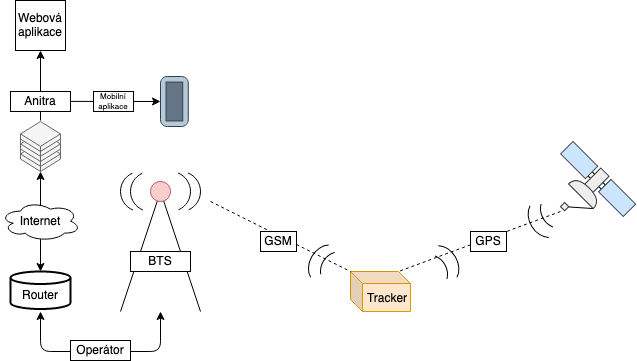
\includegraphics[width=\linewidth]{img/diagram_system.png}
	\caption{Schéma systému GPS-GSM trackerů}
	\label{fig:boat1}
\end{figure}
%%% Fiktivní kapitola s ukázkami sazby

\chapter{Existující řešení}

Tato kapitola se věnuje popisu již existujících řešení problémů nastíněných v předchozí kapitole. V této kapitole budou zhodnoceny i další problémy, např. administrativního rázu a problémy s bezpečností dat. Za konkrétní problémy se zde řadí: uchovávání informací o jedincích (morfometricé údaje, obrázky, místo označení), uchování pozic z GPS-GSM trackeru, uchování jiných geografických informací (např. lokace hnízdiště), přehlednost dat, přenositelnost a sdílení dat. Jednotlivá řešení budou popsána, zhodnocena z pohledu vydefinovaných kritérií a na konci bude vynesen verdikt, proč bylo rozhodnuto pro vývoj mobilní aplikace nad platformou Anitra. 

% popsat, jak se současně využívá Google MyMaps, fyzický zápisník, (Anitra?), Movebank aplikace

\section{Nestrukturovaný zápis}

ruční poznámky - obrázek od D.

Nestrukturovaná data je obecné označení pro data, která se zpravidla nedají popsat exaktním formálním schématem. Nejčastěji se jedná o textové dokumenty, obrázky či jiná multimédia. Pro lidské zpracování bývají nestrukturované dokumenty přirozenější, než strukturované dokumenty s exaktním schématem. Autory nestrukturovaných dat nemusí být pouze lidé, ale pro tento kontext budou uvažovány pouze artefakty lidské činnosti.

% https://books.google.cz/books?id=CRpMH-Ui7HkC&pg=PA175&dq=nestrukturovan%C3%A1+data&hl=cs&sa=X&ved=0ahUKEwi_g7HZ4NHoAhWD2aQKHaz8CkgQ6AEIKDAA#v=onepage&q=nestrukturovan%C3%A1%20data&f=false

Metoda nestrukturovaného ručního zápisu spočívá v uchovávání papírových dokumentů vznikající při činnosti ornitologů. Je možné zapsat např. pozorování jedinců, kontroly hnízd, manipulace (např. nasazení kroužku), morfometrické údaje (délky křídel), obecné poznámky. Schéma zápisu nemusí být normalizované, je zde tedy nejjednoduší možnost schéma upravit pro potřeby ornitologa, případně ornitologické organisace.

\begin{table}[h]
	\begin{tabularx}{\textwidth}{ | X | X | }
		\hline
		Kritérium                              & Hodnocení \\
 		\hline			
		Informace o jedincích                  & 1 -- absence vynuceného schématu umožňuje uložit jakékoliv informace          \\
		\hline
		Práce s pozicemi z trackerů            & 4 -- informace musí být ručně vloženy          \\
		\hline
		Práce s uživatelsky vloženými pozicemi & 3 -- informace musí být ručně vloženy, ale schéma není pevně dané          \\
		\hline
		Přehlednost dat                        & 3 -- v datech se obtížně hledá, závisí primárně na zapisovateli, některé věci nejde visualizovat jednoduše          \\
		\hline
		Přenositelnost a sdílení dat           & 4 - data jsou složitě přenositelná, mohou být i obtížně pochopitelná          \\
		\hline	
	\end{tabularx}
	\caption{Hodnocení nestrukturovaného zápisu}
\end{table}

\textbf{Výhody}

\begin{itemize}
	\item možnost kdykoliv upravit schéma,
	\item nízká náročnost na technologie,
	\item rychlost zápisu,
\end{itemize}

\textbf{Nevýhody}

\begin{itemize}
	\item obtižné vkládání fotodokumentace, o
	\item data jsou složitě přenositelná, obvykle pouze ručním přepisem do jiného systému.
\end{itemize}

\section{Strukturovaný zápis}

%https://books.google.cz/books/about/Data_informace_znalosti_a_Internet.html?id=UJh-gLdTH8IC&printsec=frontcover&source=kp_read_button&redir_esc=y#v=onepage&q&f=false stránka 2, 1.1.1

Označení \emph{strukturovaná} se přisuzuje datům, které explicitně zachycují fakta, atributy, objekty, u kterých je významným rysem existence elementů dat. Strukturované ukládání dat je strojově zpracovatelné počítači a ukládá se často v databázových systémech nebo tabulkových procesorech. V této podkapitole bude popsán zápis pomocí tabulkového procesoru.

Na rozdíl od ručního zápisu je zde možné vynutit schéma, přehlednost i přenositelnost dat je tedy nesrovnale vyšší. Změny schématu pro zaznamenání nového druhu informací mohou být komplikací, např. v případu rozdělení datového elementu na dva, nutnosti změnit procesy či procedury zapisování záznamu. Problematické je vkládání a zobrazování některých telemetrických dat z trackerů umístěných na zvířatech. Ačkoliv např. zobrazení numerických telemetrických dat (teplota, napětí na akumulátoru) je jednoduché a dá se v tabulkovém procesoru zobrazit jednoduše, geografické pozice nikoliv. Problém také nastává při přibývání dat s výkonem. Problém zde může nastat při spolupráci více uživatelů najednou, synchronizace dat se musí kontrolovat, aby nedošlo ke ztrátě dat.

\begin{table}[h]
	\begin{tabularx}{\textwidth}{ | X | X | }
		\hline
		Kritérium                              & Hodnocení \\
		\hline			
		Informace o jedincích                  & 2 -- způsob dostačuje, ale změna schématu nemusí vždy být flexibilní          \\
		\hline
		Práce s pozicemi z trackerů            & 3 -- informace musí být ručně vloženy, případně integrovány službou          \\
		\hline
		Práce s uživatelsky vloženými pozicemi & 3 -- informace musí být ručně vloženy, ale schéma není pevně dané          \\
		\hline
		Přehlednost dat                        & 2 -- v datech se dá vcelku dobře hledat, ale některé metriky je obtížné visualizovat          \\
		\hline
		Přenositelnost a sdílení dat           & 3 - data jsou přenositelná do jiných formátů, ale díky absenci standardizovaného schématu se vždy musí data napárovat ručně, sdílení dat je jednoduché          \\
		\hline	
	\end{tabularx}
	\caption{Hodnocení strukturovaného zápisu}
\end{table}

\textbf{Výhody}

\begin{itemize}
	\item možnost kdykoliv upravit schéma,
	\item nízká náročnost na technologie,
	\item rychlost zápisu,
	\item integrované visualizační nástroje,
	\item tabulková podoba dat srozumitelná pro vědce.
\end{itemize}

\textbf{Nevýhody}

\begin{itemize}
	\item závislost na přístupu k souborům tabulkového procesoru,
	\item obtížné či neefektivní zachycení nestrukturovaných dat (obrázků, volných textů),
	\item data jsou stále z větší části vkládaná ručně,
	\item data jsou složitě přenositelná, obvykle pouze ručním přepisem do jiného systému.
\end{itemize}

\section{Geografické informační systémy}

% https://www.gartner.com/en/information-technology/glossary/geographic-information-systems-gis

Geografický informační systém je označení pro sadu hardware, software a geografických dat pro sbět, správu, analýzu a zobrazení všechn způsobů geograficky referencovaných informací, neboli také prostorových dat\todo{ref}. Z geografické povahy dat tedy vyplývá, že některé GIS softwary by mohly být pro ornitologickou aplikaci vhodné. 

\subsection{Google MyMaps}

% - obrázek od D.

Google MyMaps je produktem z portfolia mapových produktů společnosti Google. Google MyMaps slouží především k uchování bodů, čar a polygonů v mapě. Pro ukládání dat tabulkového charakteru má aplikace podporu pouze pro objekty viditelné v mapě ve formě atributu, výhodou je ale jim možnost definovat schéma. Software ze své obecné charakteristiky má vysokou míru personalizace a obecnosti. Nespornou výhodou je napojení na ekosystém Google Drive, který umožňuje nahradit nedostatky této aplikace jinými. Správa příloh je zde taktéž vyřešena velmi dobře.

\begin{table}[h]
	\begin{tabularx}{\textwidth}{ | X | X | }
		\hline
		Kritérium                              & Hodnocení \\
		\hline			
		Informace o jedincích                  & 5 -- veškeré informace se vztahují k bodům, lze kategorizovat pouze jednodimenzionálně pomocí vrstev, které nemají metainformace          \\
		\hline
		Práce s pozicemi z trackerů            & 3 -- pozice musí být ručně vloženy ve formátu KML          \\
		\hline
		Práce s uživatelsky vloženými pozicemi & 1 -- vysoká míra personalizace, v podstatě universální          \\
		\hline
		Přehlednost dat                        & 2 -- mapová data lze ukládat vysoce přehledně za použití personalizace, informace k objektům v mapě jsou dostupná v tabulkovém editoru          \\
		\hline
		Přenositelnost a sdílení dat           & 2 - data lze jednoduše vyexportovat do standardního formátu KML          \\
		\hline	
	\end{tabularx}
	\caption{Hodnocení Google MyMaps}
\end{table}

\textbf{Výhody}

\begin{itemize}
	\item vysoká míra personalizace,
	\item jednoduchost softwaru,
	\item standardizovaný formát pro export i import dat (KML),
	\item napojení na ekosystém Google Drive.
\end{itemize}

\textbf{Nevýhody}

\begin{itemize}
	\item zaměřeno především na objekty v mapě,
	\item složité vytváření struktur nad objekty v mapě (taxonomie, metainformace),
\end{itemize}

%\subsection{ArcGIS}

%tady nevím, co napíšu :) nic o něm nevím

\section{Specializovaný software}

Specializované softwarové produkty vyvíjené přímo pro doménu ornitologie mohou kombinovat přístupy GISových aplikací i tabulkových procesorů, případně i dokumentových nástrojů. % víc

\subsection{Movebank}

Movebank je specializovanou aplikací vyvinutou Max Planck institutem v Německu. Aplikace se zabývá ukládáním dat o zvířatech, ať již pozičních, senzorických i vygenerovanými uživateli (např. pozorování). Aplikace není vyvinuta primárně pro ornitologické potřeby, ale její datový model obsahuje desítky datových položek vhodných pro ornitology. Značnou výhodou je podpora výrobců trackerů pro kontinuální export dat přímo do Movebank a možnost data z Movebank exportovat, či využít v doménově specickém softwaru. Za nevýhodu pro některé ornitology může být nutnost data uveřejnit, případně o ně po 90 dnech přijít. Movebank taktéž obsahuje funkce pro správu projektů a publikování studií a je mezi ornitology často citovaným zdrojem.

%https://www.movebank.org/cms/movebank-content/studies-page#owner_defined_details


\begin{table}[h]
	\begin{tabularx}{\textwidth}{ | X | X | }
		\hline
		Kritérium                              & Hodnocení \\
		\hline			
		Informace o jedincích                  & 1 --           \\
		\hline
		Práce s pozicemi z trackerů            & 1 -- aplikace přímo optimalizovaná pro tyto účely          \\
		\hline
		Práce s uživatelsky vloženými pozicemi & 2 -- ?          \\
		\hline
		Přehlednost dat                        & 1 -- platforma uzpůsobena pro prohlížení dat          \\
		\hline
		Přenositelnost a sdílení dat           & 2 -- data jsou vysoce přenositelná a dobře sdílená, problémem však je nutnost data publikovat          \\
		\hline	
	\end{tabularx}
	\caption{Hodnocení Movebank}
\end{table}

\textbf{Výhody}

\begin{itemize}
	\item doménová specializace,
	\item dlouholetý vývoj aplikace -- komplexní datový model,
	\item komplexní možnosti publikování dat,
	\item dobrá integrace s doménově specifickými nástroji
\end{itemize}

\textbf{Nevýhody}

\begin{itemize}
	\item nutnost data vždy v určité formě publikovat.
\end{itemize}

\subsection{Movebank Animal tracker}

Od tvůrců aplikace Movebank pochází i mobilní aplikce \emph{Animal tracker}, která umožňuje zobrazení tras od jednotlivých trackerů i zobrazení informací o zvířeti, co tracker nosí. Aplikace nevyžaduje žádné přihlašovací údaje a umožňuje veřejnosti nahlásit pozorování konkrétních jedinců. Za největší slabinu aplikace se dá považovat nutnost připojení k internetu, aplikace si neukládá informace do mezipaměti. Pro hledání jedinců v oblasti nižší kvality signálu tedy aplikace není vhodná. Aplikace je ale jinak velmi přehledná i rychlá. Pro aplikaci nebude uvedeno vlastní hodnocení, jelikož se jedná o rozšíření zmíněné aplikace Movebank pro mobilní zařízení.

\begin{figure}[h]
	\begin{center}
		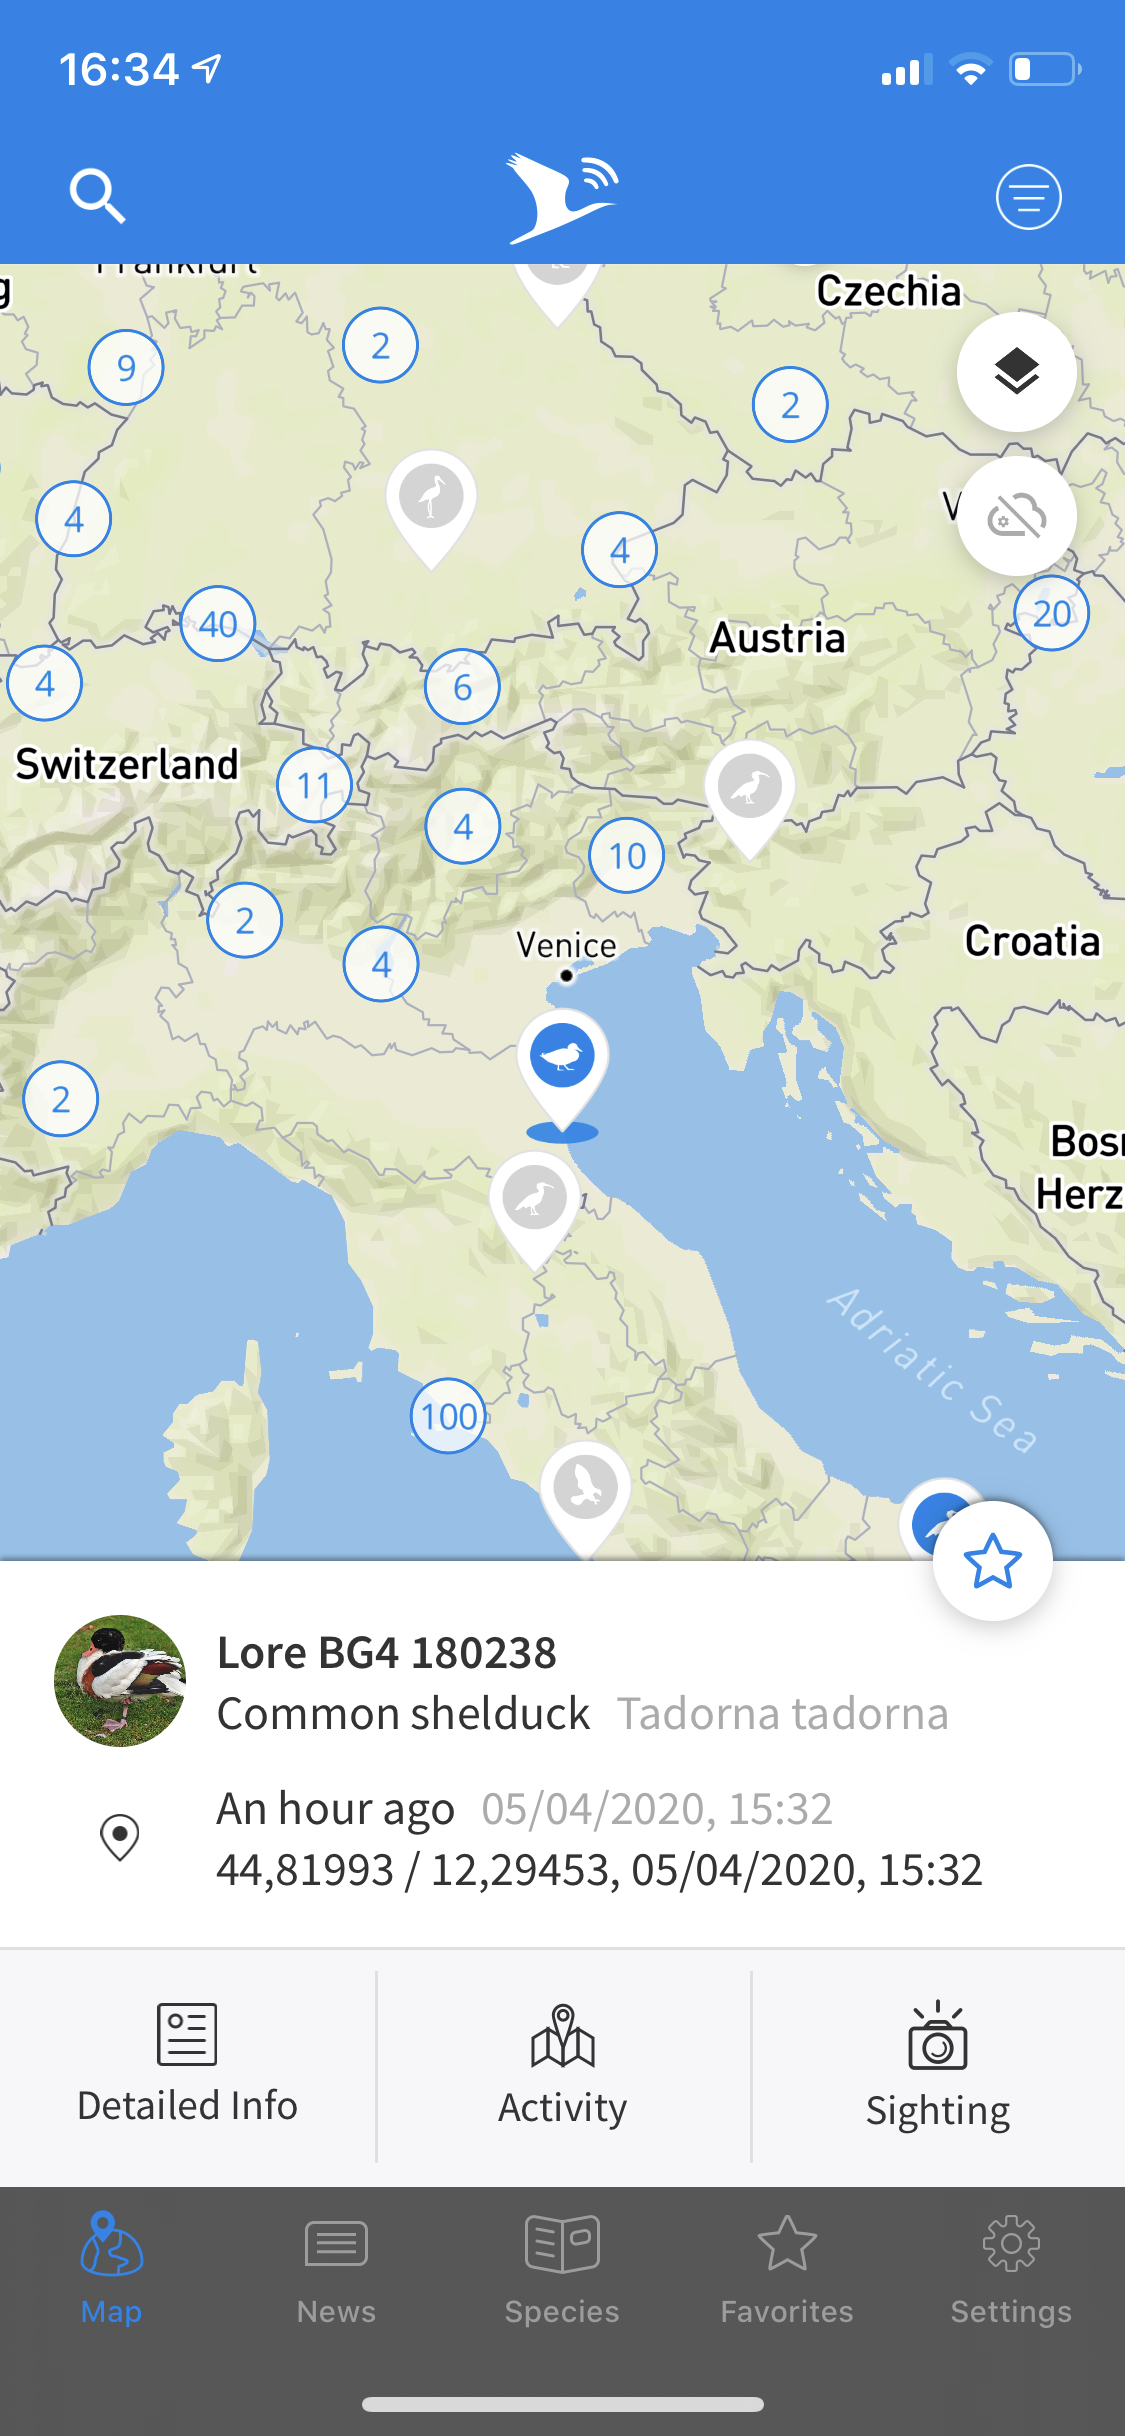
\includegraphics[width=70mm]{img/animaltracker_app_movebank.png}
	\end{center}
	\caption{Screenshot z aplikace Movebank Animal Tracker}
	\label{fig:movebank}
\end{figure}


\subsection{Anitra}

Anitra je českou ornitologickou značkou zabývající se vývojem a produkcí vlastních GPS-GSM trackovacích zařízení a poskytování softwarové platformy pro zobrazení dat a správu projektů. Rozdílem oproti platformám jiných výrobců je od základu jiná koncepce platformy. Platforma poskytovaná firmou Anitra průběžně integruje data z GPS-GSM trackerů od více výrobců a umožňuje nad daty dělat analýzy, automaticky je zpracovat dle předem stanovených pravidel, spravovat informace o jedincích, zadávat do aplikace vlastní body a přílohy. Od předem zmiňovaného Movebanku se aplikace liší především v možnosti ochranně vlastnictví dat, v aplikaci Anitra není povinnost data kdykoliv publikovat a majiteli dat zůstávají uživatelé. Aplikace taktéž umožňuje generovat uživatelsky přívětivé výstupy pro veřejnost či filtrovaná nebo plná data jednoduše sdílet mezi uživateli. Za podstatnou nevýhodu a nutnost využívat alternativní způsob zápisu v poli je především fakt, že platforma Anirta je řešena jako webová aplikace. V mobilních zařízeních je tedy obtížněji použitelná, ale hlavní nevýhodou je nutnost být stále připojen k internetu.

\begin{table}[H]
	\begin{tabularx}{\textwidth}{ | X | X | }
		\hline			
		Kritérium                              & Hodnocení \\
		\hline			
		Informace o jedincích                  & 1 -- detailní schéma vhodné pro ukládání informací o zvířatech          \\
		\hline
		Práce s pozicemi z trackerů            & 1 -- aplikace přímo optimalizovaná pro tyto účely          \\
		\hline
		Práce s uživatelsky vloženými pozicemi & 1 -- modul aplikace věnovaný pro vytváření těchto objektů          \\
		\hline
		Přehlednost dat                        & 1 -- data lze zobrazit v mapě, tabulce, vyexportovat          \\
		\hline
		Přenositelnost a sdílení dat           & 1 -- vlastník může vždy data vhodně vyexportovat          \\
		\hline	
	\end{tabularx}
	\caption{Hodnocení Anitra}
\end{table}

\textbf{Výhody}

\begin{itemize}
	\item doménová specializace,
	\item dynamický rozvoj aplikace,
	\item 
\end{itemize}

\textbf{Nevýhody}

\begin{itemize}
	\item webová aplikace není vhodná pro použití v terénu,
	\item platforma není mezi ornitology příliš rozšířená,
	\item proprietární a nezdokumentované API.
\end{itemize}


%%% Fiktivní kapitola s ukázkami sazby

\chapter{Analýza požadavků}

Kapitola analýza požadavků se věnuje první fázi ve vývoji softwarového projektu. Analýza požadavků se skládá z různých fází dle použité metodiky, ale vždy je cílem od relevantních stran získat seznam požadavků, co aplikace musí splňovat, aby naplnila cíle, kvůli kterým se k vývoji SW projektu rozhodlo. V jiných slovech je tedy část analýzy požadavků kritická pro úspěch softwarového projektu \cite{maguire2002user}.

% chce to zdroje, a ten text je taky dost divný

\section{Identifikace stakeholderů}

% vysvětlit pojem stakeholder, jak se dělá analýza stakeholderů

Identifikace stakeholderů je první fází v analýze požadavků. Účelem této fáze je identifikovat všechny relevantní zúčastněné strany, aby mohly být zapojeny do fáze sběru požadavků a přiřadit k nim jednotlivé případy užití aplikace \cite{maguire2002user}. V případě nedostatečného zapojení stakeholderů je vysoká pravděpodobnost, že software nebude uspokojovat potřeby všech zúčastněných stran.

Za stakeholdery byly identifikovány následující subjekty: stávající uživatele webové aplikace Anitra a majitel firmy Anitra System s.r.o.

Stávající uživatelé aplikace již požadovali funkce pro práci v terénu a jejich požadavky byly zaevidovány do pořadníku funkcí pro webovou aplikaci. Tyto požadavky byly konzultovány se zakladatelem firmy Anitra a byly vybrány k řešení. Zakladatel firmy je projektovým manažerem a komunikuje se zákazníky na denní bázi, má tedy dostatečný přehled o požadavcích zákazníků a jejich priorit, zároveň působí i jako kontaktní bod podpory pro aplikaci. Cílem zakladatele firmy je poskytnout uživatelům nástroje pro efektivní práci v terénu i pro rychlou kontrolu dat z mobilních zařízení, což by mohlo být bráno jako konkurenční výhoda, jelikož na trhu nebyla nalezena podobná aplikace.

\section{Sběr požadavků}

Pro zakladatele firmy Anitra je cílem mobilní aplikace doplnění ekosystému značky Anitra o vhodné řešení zobrazení a zadávání dat v terénu. Na začátku práce byla pouze dostupná webová aplikace, která měla pro práci v terénu následující nevýhody:

\begin{itemize}
	\item data po odpojení z internetu nebyla dostupná, ve většině případů ani již načtená data,
	\item aplikace byla příliš náročná na energii,
	\item mapové podklady se nezobrazovaly po odpojení ze sítě,
	\item aplikace byla na datový přenos příliš náročná,
	\item navigace v GUI byla pro malá zařízení příliš složitá.
\end{itemize}

Tyto podněty byly sebrány od uživatelů webové aplikace Anitra v období 2018-2020, ale mělo by se jednat o dostatečný základ pro zařazení mobilní aplikace do portfolia ekosystému Anitra, jelikož se jedná o obecné předpoklady pro software tohoto typu.

Z těchto zkušeností uživatelů vyplynuly klíčové funkční i nefunkční požadavky na funkcionalitu aplikace. Jednotlivé části jsou rozebrány níže. Další funkční požadavky byly definovány zakladatelem firmy Anitra (zde uvedeny ve zkrácené formě, seřazeny dle priority):

\begin{itemize}
	\item zobrazit poslední polohu zařízení v mapě,
	\item možnost stáhnout si mapy před kontrolou na místě,
	\item zobrazení dat ze zařízení,
	\item zobrazení vlastní pozice na mapě
	\item notifikace o nových datech,
	\item zaznamenat trasu, bod,
	\item možnost přiložit obrázek k zvířeti.
\end{itemize}

\section{Funkční požadavky}

Funkční požadavky popisují očekávané chování systému, ale nevěnují se technickým detailům, jak má systém fungovat. Funkční požadavky slouží pro splnění potřeby uživatelů a lze je vyjádřit ve formě případů užití nebo diagramu případu užití \cite{jacobson1987object}.

Jednotlivé případy užití jsou rozebrány v kapitole uvedené níže.

\subsection{Diagram případů užití}

Diagram případu užití je diagramem ze standardní sady UML využívané v softwarovém inženýrství.

\begin{figure}[H]
	\begin{center}
		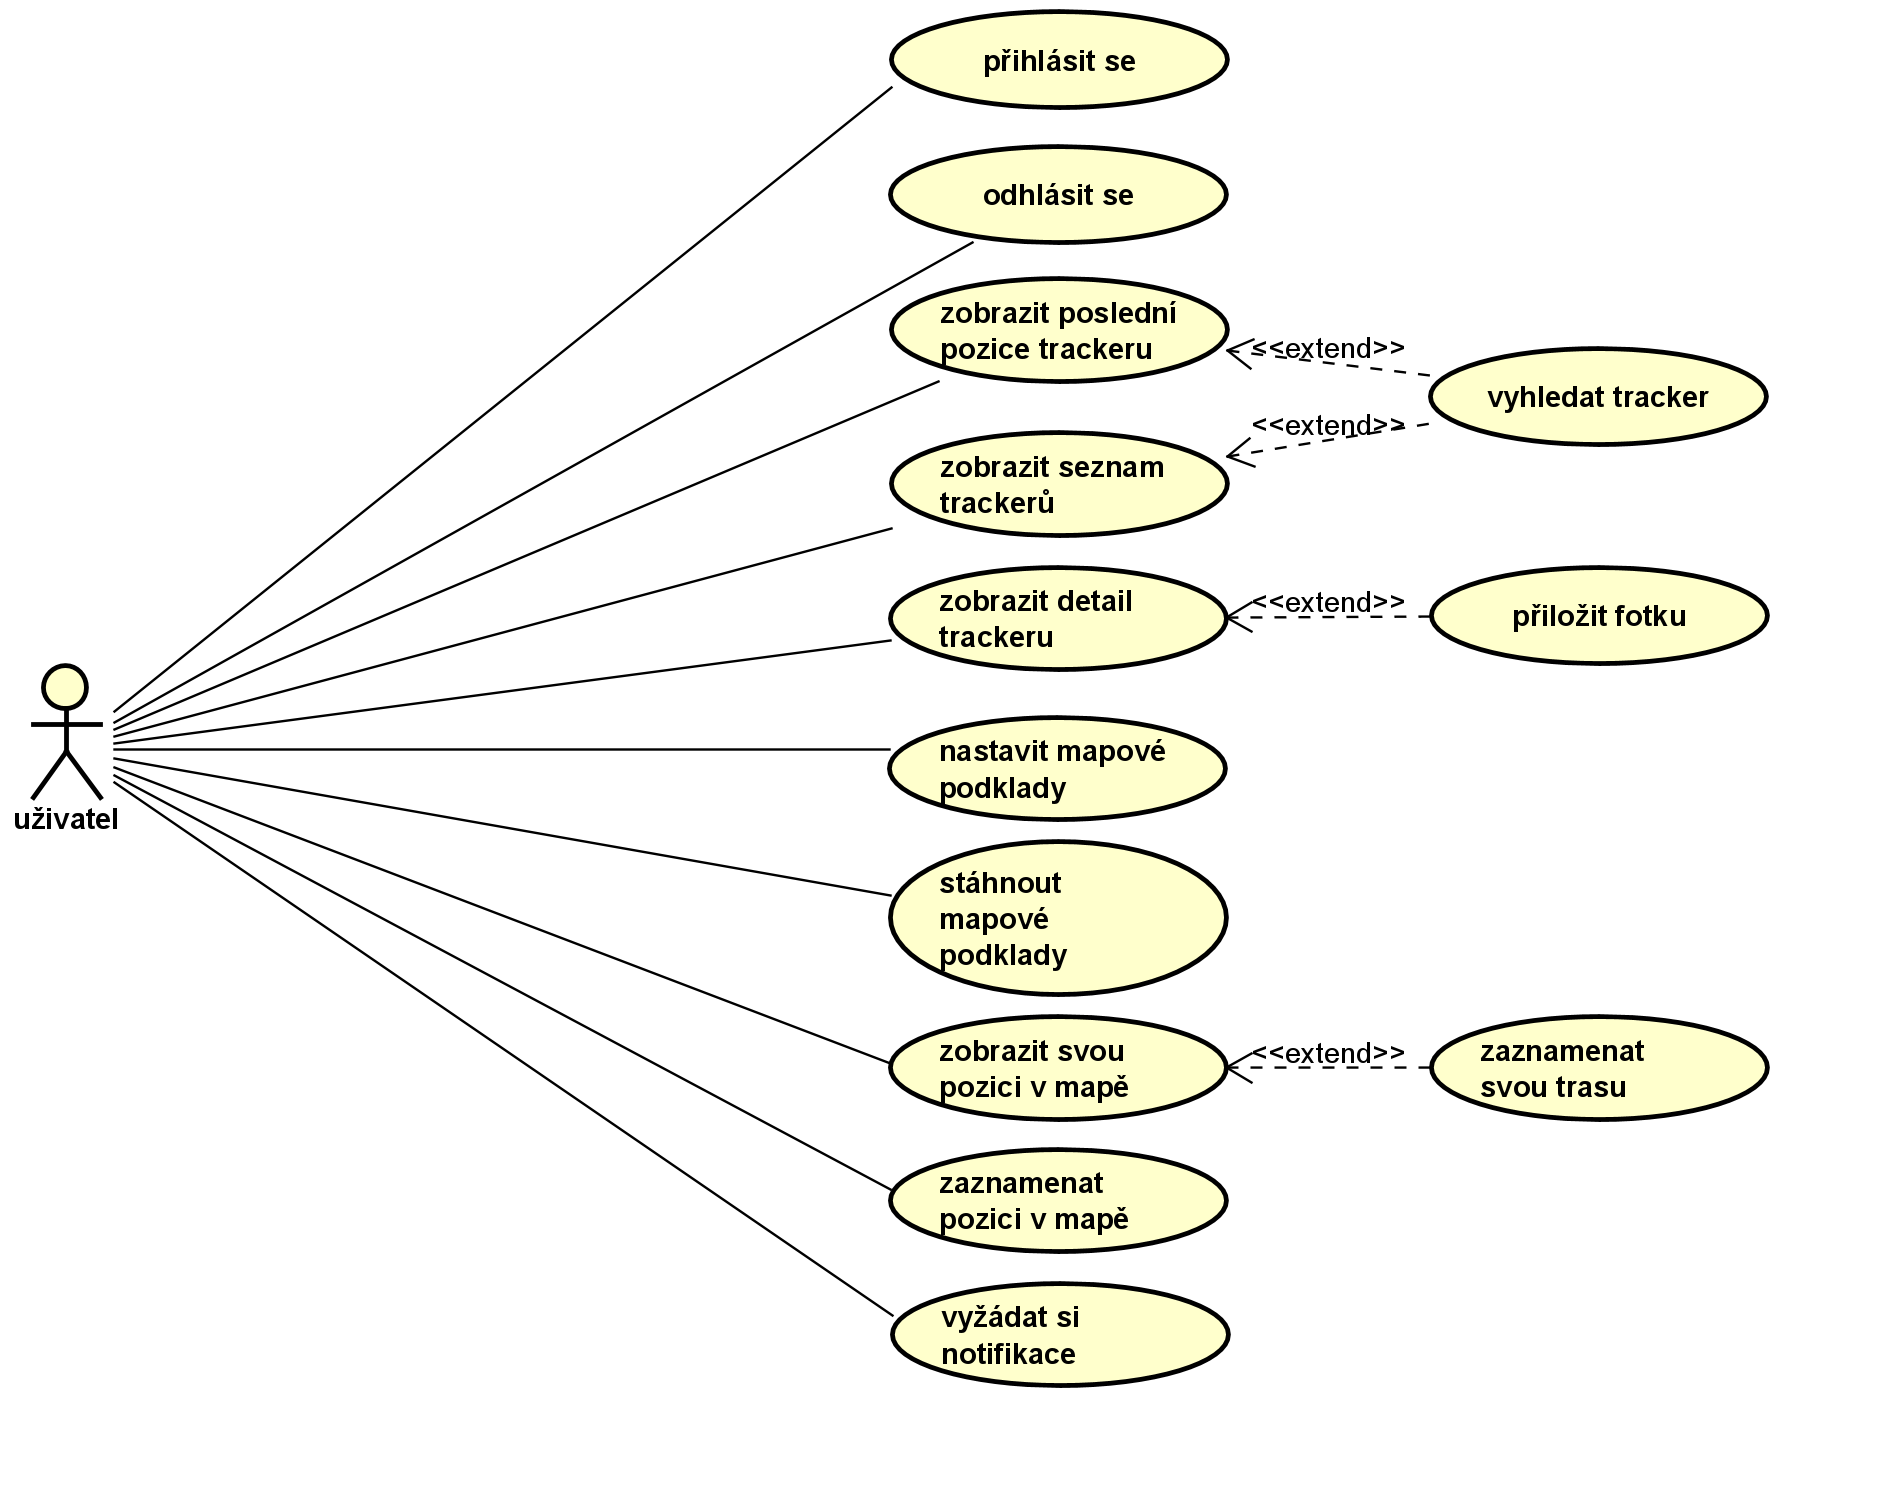
\includegraphics[width=140mm]{img/usecase.png}
	\end{center}
	\caption[Diagram případu užití]{Diagram případu užití -- zdroj: autor}
\end{figure}

Diagram případů užití byl sestaven dle nasbíraných požadavků zmíněných v minulé kapitole. Případy užití byly rozšířeny o nevyslovené, ale odvoditelné požadavky, např. možnost přihlásit se a odhlásit se.

\section{Nefunkční požadavky}

Nefunkční požadavky udávají kvalitu systému, ale ne jeho chování. Tyto požadavky často přináší omezení do implementací funkčních požadavků a je někdy obtížné tyto požadavky sladit, mohou působit i protichůdně. Jako příklad se často uvádí požadavky spojené s komfortem uživatelů (např. přístupnost, výkonnost, lokalizace), provozem aplikace (přenositelnost, tolerance chyb) a bezpečnost. Do nefunkčních požadavků se řadí i požadavky související s možností dalšího vývoje systému \cite{chung2012non}.

Z výše uvedeného seznamu požadavků vyplynulo několik klíčových nefunkčních požadavků především ve vztahu k uživatelům. Pro úspěch aplikace je nutné, aby grafické rozhraní aplikace bylo dostatečně jednoduché a podstatné funkce byly rychle přístupné bez složitých navigací, jelikož uživatel nemusí mít mnoho času pro práci s aplikací v terénu. S tímto souvisí i nutnost odezvy v jednotkách sekund. 

Neuvedeným požadavkem je multiplatformnost aplikace, jelikož část uživatelů stávající aplikace využívá mobilní operační systém iOS a část Android. Podstatným požadavkem je i rozšiřitelnost aplikace, jelikož se s vývojem aplikace počítá i po dokončení této práce.

\section{Časové aspekty}

Aplikace má být vyvinuta a nasazena nejpozději do konce května, ideálně již v dubnu. V tuto dobu probíhá nejvyšší počet ornitologických operací spojených s nasazováním trackerů, kontrolou hnízd a dalších. Aplikaci nebylo možné začít vyvíjet dříve než v polovině února kvůli návaznosti na API již existující webové aplikace. Pro prvotní verzi aplikace je kritické aby spolehlivě zobrazovala poslední body v mapě a po prvotní synchronizaci fungovala bez internetového připojení.

%%% Fiktivní kapitola s ukázkami sazby

\chapter{Technologie}

Kapitola technologie se zabývá využitými technologiemi a jakým způsobem byly vybrány. Jednotlivé technologie jsou představeny pro porozumění následující kapitole návrh, který byl proveden s ohledem na vybrané technologie.

Pro výběr technologií byla stanovena následující kritéria:

\begin{itemize}
	\item podpora platforem iOS a Android,
	\item rychlost vývoje,
	\item velikost komunity a aktuálnost dokumentace,
	\item programovací jazyk,
	\item jednoduchost vytváření UI,
	\item dostupnost potřebných komponent pro aplikaci.
\end{itemize}

Jednotlivá kritéria jsou rozebrána níže.

% vlastní oddělení

\section{Kritéria výběru}

\subsection{Podpora více platforem}

Podpora platforem iOS a Android je kritickým požadavkem aplikace vycházející z analýzy požadavků. Technologie musí podporovat, ideálně platformně nezávisle abstrahovat, přístup k zdrojům souborového systému, přístup k vzdáleným zdrojům pomocí protokolu HTTP, umožnit vytvářet mapové aplikace, bezpečně uložit uživatelské přihlašovací údaje. Technologie by neměla vyžadovat platformně závislý nativní kód.

\subsection{Rychlost vývoje}

Rychlost vývoje je obtížně kvantifikovatelnou veličinou. Do rychlosti vývoje lze zahrnout mnoho aspektů a záleží, z jakého pohledu se na problematiku pohlíží. Z pohledu řízení projektu se může např. jednat o počet dostupných vývojářů a doba adaptace na technologii. Z pohledu programátora se může jednat o kvalitu a dostupnost vývojových nástrojů, dostupnost knihoven, přehlednosti kódu, dostupné funkce programovacího jazyka technologie. Z pohledu údržby se může jednat o očekávanou životnost technologie nebo dostupnosti testovacích nástrojů. Kombinací těchto aspektů může vzniknout více či méně subjektivní hodnocení, jak rychlý by měl vývoj s pomocí danou technologií být. Neexistuje žádná konkrétní metodika, která by se snažila tento jev kvantifikovat, ale existují názory mezi odbornou veřejností, které technologie se považují za vhodné pro rapidní vývoj. Pro tuto práci, z hlediska časového, bude nutné vybrat technologii, která naplňujne co nejvíce kritérií pro rapidní vývoj.

\subsection{Velikost komunity}

Velikost komunity určuje dvě podstatné věci -- životnost technologie a množství dostupné aktuální dokumentace a komunitních návodů. Pro dlouhodobé hledisko je potřeba vybrat technologii, která se dle současného stavu zdá dlouhodobě perspektivní a ne na úpadku. Dostupná kvalitní oficiální i komunitní dokumentace je taktéž podstatným faktorem, který technologii zpřístupňuje pro nové projekty. Tato veličina je již kvantifikovatelná např. analýzou trendů či sledováním open-source projektů v daných technologiích. Pro určení této veličiny bude provedeno srovnání dle Google Trends a hlavních repozitářů

\subsection{Programovací jazyk}

Programovací jazyk technologie je taktéž podstatný faktor. Standardní knihovny některých jazyků mají mnoho dostupných funkcí, které urychlují nebo komplikují vývoj. např. již předpřipravené metody pro HTTP komunikaci. Některé jazyky mohou těžit i z vlastností dané svým paradigmatem, např. funkcionální jazyky mohou být vhodnější pro paralelní zpracování. Aspekty paralelního nebo asynchronního zpracování jsou pro mobilní aplikace podstatné z důvodu nezamknutí vykreslovacího vlánka pro uživatelské rozhraní z důvodu uživatelského komfortu.

\subsection{Vytváření uživatelského rozhraní}

% https://developer.mozilla.org/en-US/docs/Web/CSS/CSS_Flexible_Box_Layout/Basic_Concepts_of_Flexbox
Aspekty vytváření uživatelského rozhraní spočívají především v možnostech technologie. Technologie by měla umožnit vytvářet reaktivní a moderně vypadající uživatelská rozhraní, podporovat animace, reagovat na uživatelské interakce. Na těchto principech je založen například Material Design od společnosti Google. Výhodou nástroje pro vytváření uživatelského rozhraní je moderní přístup k vytváření uživatelského rozhraní např. s tzv. \emph{flexboxem}, nástrojem pro jednodimenzionálně řazená uživatelská rozhraní s rožšířenou podporou zarovnání \cite{FlexboxMDN}. Nativní podpora stylování v podobě webových CSS je taktéž vyhodou, jelikož ji nezanedbatelná vývojářů do jisté míry rozumí.

\subsection{Hotové komponenty}

Hotové komponenty umožňují se při vývoji věnovat pouze řešení potřebných doménových problémů, namísto vytváření od základu nových komponent a s tím spojené testování. Důsledkem je využívání specifického portfolia komponent, na kterých může vývojář nabrat znalosti a použít je na dalším projektu využívající stejnou technologii, případně vývojář již zkušenosti mít může, tím vývoj výrazně urychlit. Hotové komponenty jsou obrovskou výhodou v rapidním prototypování, protože mohou aplikaci již ve fázi prototypu poskytnout určitou představu o finální funkčnosti.

\section{Výběr technologie}

% jak? byly vybrány technologie

Pro užší posouzení byly vybrány následující technologie: React Native, Xamarin a Flutter. Technologie jsou ve zkratce popsány níže a zhodnoceny.

\begin{figure}[h]
	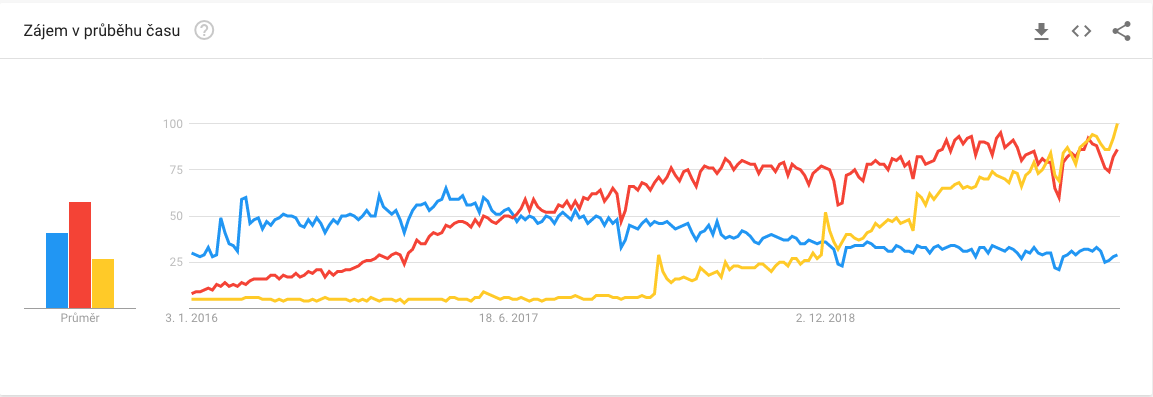
\includegraphics[width=\linewidth]{img/google_trends.png}
	\caption[Srovnání trendů technologií pro mobilní vývoj]{Srovnání trendů v období 1. 1. 2016 až 11. 4. 2020; červená křivka -- React Native, modrá křivka -- Xamarin, žlutá křivka -- Flutter; -- Zdroj: Google Trends}
	\label{fig:gtrends}
\end{figure}

\subsection{Hodnocení React Native}

%https://github.com/facebook/react-native
% http://pypl.github.io/PYPL.html
React Native je framework pro vytváření nativních mobilních aplikací s JS frameworkem React. React Native je uveden v další kapitole. Tento framework byl vybrán k posouzení především kvůli obrovské komunitě a prověřenosti. Nespornou výhodou frameworku využití jazyku JavaScript, který je třetím nejvíce vyhledávaným programovacím jazykem. JavaScript (resp. EcmaScript) je uveden v následujících kapitolách a nebudou zde jeho výhody rozvedeny. Pod pojmem React Native je zde brána v potaz nadstavba Expo, která dále abstrahuje od nativního kódu.

\begin{table}[H]
	\begin{tabularx}{\textwidth}{| X | X | X |}
		\hline
		Kritérium                       & Hodnocení & Poznámka \\
		\hline
		Podpora platforem  & 2  & plně podporuje obě mobilní platformy, ale některá API jsou dostupná pouze pro jednu \\
		\hline
		Rychlost vývoje                 & 1 & kombinace jednoduchého jazyka, dobrých nástrojů a dostupných knihoven \\
		\hline
		Velikost komunity a dokumentace & 1  & z obrázku  \ref{fig:gtrends}  vyplývá obrovská popularita frameworku v posledních 3 letech \\
		\hline
		Programovací jazyk              & 1 &          \\
		\hline
		Vytváření UI                    & 2 &          \\
		\hline
		Hotové komponenty               & 1 & 24299 balíčků \footnote{\href{https://www.npmjs.com/search?q=react\%20native} k 11. 4.}   \\
		\hline
	\end{tabularx}
	\caption{Hodnocení React Native}
\end{table}

\subsection{Hodnocení Xamarin}

% https://dotnet.microsoft.com/apps/xamarin

Xamarin je rozšíření platformy .NET pro vývoj multiplatformních aplikací nejen pro mobilní zařízení. Xamarin je postavený nad návrhovým vzorem Model-View-ViewModel, který odděluje uživatelské rozhraní, data a aplikační logiku do separátních vrstev. Uživatelské rozhraní je možno vytvářet deklarativně v jazyku XAML, případně v přímo v jazyku C\#. Změny v uživatelském rozhraní se zajišťují pomocí tzv. data bindingu, tedy navázání proměnné v uživatelském rozhraní s proměnnou ve view modelu. Za Xamarinem stojí technologický gigant Microsoft a je z vybraných technologií nejstarší.

\begin{table}[H]
	\begin{tabularx}{\textwidth}{| X | X | X |}
		\hline
		Kritérium                       & Hodnocení & Poznámka \\
		\hline
		Podpora platforem & 2 &          \\
		\hline
		Rychlost vývoje                 & 3 &          \\
		\hline
		Velikost komunity a dokumentace & 3 &          \\
		\hline
		Programovací jazyk              & 2 &          \\
		\hline
		Vytváření UI                    & 2 &          \\
		\hline
		Hotové komponenty               & 4 & \\
		\hline
	\end{tabularx}
	\caption{Hodnocení Xamarin}
\end{table}

\subsection{Hodnocení Flutter}

%https://github.com/flutter/flutter

Flutter je SDK od společnosti Google sloužící pro vytváření "nádherných, rychlých zážitků pro mobil, web a desktop s jedním zdrojovým kódem". Flutter je z vybraných technologií nejnovější, ale výrazně nejrychleji roste. Za obrovskou výhodu Flutteru se dá považovat vývojové prostředí s funkcemi live-reload, které na rozdíl od vývojových prostředí pro Xamarin a React Native má výrazně lepší zapamatování stavu. Flutter byl přímo navržen pro aplikace tohoto typu a obsahuje tedy mnoho optimalizací. Flutter aplikace jsou taktéž výrazně menší na stáhnutí, než aplikace React Native nebo Xamarin. Za nevýhodu Flutteru se dá považovat pouze jazyk Dart, který na rozdíl od C\# nebo JS není stále dostatečně viditelný ve vývojářské komunitě. Podstatnou nevýhodou je nízký počet komponent, vývojáři si tedy musí značnou část komponent psát sami.

\begin{table}[h]
	\begin{tabularx}{\textwidth}{| X | X | X |}
		\hline
		Kritérium                       & Hodnocení & Poznámka \\
		\hline
		Podpora platforem               & 1 &          \\
		\hline
		Rychlost vývoje                 & 1 &          \\
		\hline
		Velikost komunity a dokumentace & 3 &          \\
		\hline
		Programovací jazyk              & 4 &          \\
		\hline
		Vytváření UI                    & 1 &          \\
		\hline
		Hotové komponenty               & 3 & 8450 balíčků \footnote{https://pub.dev/flutter/ k 11. 4.} \\
		\hline    
	\end{tabularx}
	\caption{Hodnocení Flutter}
\end{table}

\textbf{Výhody}

\begin{itemize}
	\item dynamická technologie,
	\item vysoce kvalitní vývojářské nástroje,
	\item vývíjeno stejnou společností, která stojí za OS Android,
	\item vysoká míra optimalizace,
	\item možnost vytvářet i webové aplikace.
\end{itemize}

\textbf{Nevýhody}

\begin{itemize}
	\item relativně obskurní jazyk Dart,
	\item nížký počet aktuálních návodů,
	\item nížký počet relevantních komponent,
	\item obtížnější zprovoznění + velikost SDK,
	\item komunita nemá stále stejnou velikost jak komunita React a React Native.
\end{itemize}

\subsection{Vybraná technologie}

Pro řešení práce byla vybraná technologie React Native (resp. Expo), jelikož ze srování vyšla nejlépe. Dále bylo rozhodnuto o využití nadstavby TypeScript na JS a správce stavů MobX. Popis technologie je uveden v další kapitole.

\section{React Native}

Technologie React Native je postavena na mnoha dílčích částech, které se musí uvést pro komplexní pochopení React Native samotného.

\subsection{JavaScript a EcmaScript}

% https://www.computerworld.com/article/3458282/the-a-z-of-programming-languages-javascript.html
% https://web.archive.org/web/20150910072359/http://adaptivepath.org/ideas/ajax-new-approach-web-applications/
% https://github.com/nodejs/node-v0.x-archive/tags?after=v0.0.4
% https://github.com/angular/angular.js/releases?after=v0.9.4

JavaScript je multiparadigmatický interpretovaný slabě typovaný programovací jazyk určen primárně pro webové prohlížeče. JavaScript vznikl v roce 1995 Brendanem Eichem pod firmou Netscape. Cílem bylo přidat interaktivitu do čistě statických webových stránek a reagovat tedy na interakci uživatele i jinak, než jen přenačtením celé stránky. S obrovským rozvojem domacích počítačů přišel i rozvoj internetu a internetových prohlížečů. Od již zmíněného roku 1995 do roku 2004 byl trh webových prohlížečů dominován verzemi prohlížeče Internet Explorer od firmy Microsoft, která přišla s vlastní implementací JavaScriptu, tzv. JScriptem. Kvůli nespolupráci mezi vývojáři různých implementací vznikaly v jazyku nekonzistence mezi prohlížeči, ale i přesto se jazyk určitým směrem ubíral. V roce 2005 byl zaveden termín AJAX, který znamenal obrovskou změnu v interaktivitě webových aplikací. Zkratka AJAX, neboli Asynchronous JavaScript and XML byla revoluční ve změně komunikace serveru s JavaScriptem. JavaScript dříve obdržoval fragmenty HTML od serveru a tím aktualizoval stránku, případně se stránka po každé významné interakci uživatele překreslila sama. AJAX zavedl možnost jak na pozadí získat z určitých vstupů určité výstupy v lépe strojově zpracovatelném formátu. S tímto revolučním nápadem začaly vznikat první JavaScript knihovny a frameworky pro interaktivní webové \emph{aplikace}, např. dodnes používaná knihovna jQuery. Dalším podstaným krokem byl vývoj webového prohlížeče Google Chrome, resp. jeho JavaScript interpreteru V8. V8 je open-source JS interpreter s just-in-time kompilací, který byl revoluční primárně ve své rychlosti. Tento interpreter byl také zařazený i do aplikací mimo webové prohlížeče, čímž se případy užití pro jazyk výrazně rozšířily. Zde za zmínku stojí node.js (vznik datovaný do roku 2009) a jeho ekosystém NPM, který je rozveden níže. Dalším milníkem podstatným pro tuto práci je rozšíření frameworků pro single-page aplikace, které emulují chování běžných nativních aplikací v prohlížeči. Aplikace fungují na komponentovém systému a aktualizují se při změně dat. Aplikace jsou tedy uživatelsky i programátorsky komfortnější a jejich vývoj je značně rychlejší. Aplikace tohoto typu se rozšiřují od roku 2010.

%https://tc39.es/ecma262/#sec-overview

EcmaScript je specifikací jazyka JavaScript, kterou musí každé prostředí implementovat. EcmaScript definuje pouze jazyk, ale ne objekty kontextu, např. ve webových prohlížečích není definována interakce s DOM. JavaScript je ale dnes používán i na serverech, embedded zařízeních či jako skriptovací jazyk mnoha programů, bylo nutno od těchto specifikací abstrahovat, aby základ jazyka zůstal stejný. Tímto ale vznikají jisté nekonzistence mezi implementacemi v různých prohlížečích, obzvláště napříč verzemi, kde se jádro interpreteru již neaktualizuje. Pro řešení těchto problémů byly mimojiné zavedeny tzv. \emph{polyfilly}, které doplňují určité funkce z nové verze zpětně do staré a \emph{transpilátory} (např. Babel), které některé nové jazykové funkce umí převést do verze ES kompatibilní se starým interpreterem. V čase psaní této práce je aktuální verzí EcmaScript 2018.

S příchodem node.js ekosystému vznikl v JS světě koncept NPM balíčků. Balíčky jsou publikovány autorem do centrálního repozitáře balíčků a každý programátor si tento balíček může nainstalovat. Balíčky jsou typicky knihovny, malého či velké rázu, frameworky, nástroje, samostatné programy či kompletní projekty. Koncept balíčků výrazně urychluje vytváření projektů a instalaci knihoven. Příklady práce s NPM jsou uvedeny v kapitolách React a React Native.

\subsection{TypeScript}

TypeScript je nadstavbou jazyka ECMAScript. TypeScript rozšiřuje jazyk o kontrolu typů a běžné konstrukty známé z jiných jazyků (např. rozhraní). Jazyk je plně kompabitilní s ES, ale samotný TypeScript není přímo většinou interpeterů spustitelný. Při sestavování projektů s TypeScriptem se využívá tzv. transpilace, převedení z jednoho programovacího jazyka do druhého. TypeScript vyšel v roce 2012 pod křídly firmy Microsoft a je aktivně vyvíjen dodnes.

TypeScript se běžně využívá ve větších projektech především kvůli prevenci chyb a zvýšení přehlednosti kódu. Vývojová prostředí taktéž lépe rozumí typovaným jazykům a tímto se může i zrychlit vývoj. Zaintegrovat TypeScript do existujícího projektu také není problém, jelikož jakýkoliv validní kód v ES je validní kód v TypeScript.

\subsection{React}

\begin{figure}
	\begin{center}
		
\includegraphics[width=70mm]{img/react-logo.png}
	\end{center}
	\caption{Logo React -- zdroj: Facebook Inc.}
\end{figure}

% https://reactjs.org/

React je JS knihovna pro vytváření uživatelských rozhraní (ref) od společnosti Facebook. React je deklarativní, component-based knihovna s velkým spektrem potenciálních využití. Jako jiné moderní UI knihovny v JS je taktéž reaktivní, při změně dat se překreslí uživatelské rozhraní pouze tam, kde musí. Deklarativnost Reactu spočívá právě v zakládání si na komponentách. Uživatelské rozhraní se skládá z předdefinovaných, uživatelem vytvořených nebo komunitou vytvořených komponentách, které se do sebe skládají. Každá komponenta si uchovává vlastní data (popř. stav v atributu props) a může komunikovat s nadřazenou či podřazenou komponentou pomocí událostí nebo předáváním dat. Komponenty jsou v Reactu definovány pomocí speciální kombinace JS a HTML, tzv. JSX. JSX je vždy obaleno elementem, který může být HTML elementem či jinou komponentou. V JSX se na rozdíl od běžného HTML může vyskytovat aplikační logika, uvozena v složených závorkách.  Níže je uvedena kompletní komponenta z oficiální dokumentace (ref!), která při využití této komponenty \verb|<HelloComponent name="world"/>| vypíše do div tagu Hello world.

\begin{lstlisting}[language=JavaScript, caption=React komponenta]

class HelloMessage extends React.Component {
	render() {
		return (
			<div>
			Hello {this.props.name}
			</div>
		);
	}
}
\end{lstlisting}

Případně pro ilustraci podmíněné logiky lze uvést následující příklad:

\begin{lstlisting}[language=JavaScript, caption=React komponenta s podmínkou]

class ConditionalComponent extends React.Component {
	render() {
		return (
			<div>
				{this.props.sayHello?
					<span>
							Hello {this.props.name}
					</span>
					:<span>
							Goodbye {this.props.name}
					</span>
				}
			</div>
		);
	}
}
\end{lstlisting}

Příklad využívá slabého typování JS, stačí tedy pouze aby sayHello bylo pravdivé (případně \emph{truthy} -- aby se alespoň evaluovalo na pravdu) a provede se správná část JSX. Podmínka je zde zapsána ve formě ternárního operátoru, klasická if struktura by musela být ve vlastní funkci.

Komponenty mohou samozřejmě být výrazně komplexnější, např. mohou obsahovat funkce vracející JSX a tím být výrazně přehlednější. Mimo JSX mohou obsahovat metody a atributy pro práci s daty, např. pro získání dat ze serveru nebo k vyfiltrování dat. Tyto funkce mutují stav komponenty pomocí funkce  \verb|setState|, která mění stav komponenty ( \verb|this.props.*| v ukázce) a zároveň zajistí její překreslení, pokud je to nutné. Změna jména by tedy mohla být docílena i zavoláním \verb|this.setSate({name: 'svete'});| z metody v komponentě.

React aplikce se ale nemusí skládat jen z komponent, modulární systém nového JS umožňuje jednoduše zakomponovat do aplikace i kód mimo komponenty. Komponenty ale stále zůstanou centrálním bodem aplikace a je tedy výhodné aplikaci strukturovat do většího počtu malých komponent kvůli přehlednosti, testovatelnosti a znovupoužitelnosti.

\subsection{React Native}

React Native je framework pro vytváření mobilních aplikací postavený nad knihovnou React, opět od společnosti Facebook. React Native, na rozdíl např. od progresivních webových aplikací se chová jako nativní aplikace -- aplikace je vykreslovaná nativním kódem a nemá omezení typická pro webové aplikace, např. v přístupu k určitým API. Rozdílem od čistého Reactu je omezený výběr komponent a výrazně odlišný způsob jejich stylování. Zatímco v React je možno využít plného rozsahu CSS a všech HTML elementů, v React Native jsou v základu poskytnuty jen určité komponenty, nejpodstnější z nich jsou View, Text a Image. View je kontejnerovým prvkem, který nemá žádné specifikované využití. Používá se často pro držení jiných komponentů či stylování. Text je jediná komponenta, která může obsahovat text. Image je komponenta obsahující obrázek z lokálního nebo vzdáleného zdroje. Jsou poskytnuty i další komponenty pro formulářová pole (TextInput, Button, Picker), indikátory aktivity a seznamy. Jiné komponenty se dají složit z těchto základních komponent, jejich událostí a jejich stylů. 

% co sem dál napsat?

React Native umožňuje psát nativní kód a mnoho komponent této skutečnosti využívá. Nevýhodou tohoto přístupu je, že nativní kód se musí psát v Javě pro Android a v jazyce Swift pro iOS. Tímto vzniká prakticky vzato duplicita kódu a dvojnásobná nutnost testovat.

\subsection{MobX}

% https://books.google.nl/books?id=ALFmDwAAQBAJ&pg=PP1&lpg=PP1&dq=michel+weststrate+mobx+quick+start+guide:+supercharge+the+client+state+in+your+react+apps+with+mobx&source=bl&ots=D460fxti0F&sig=ivDGTxsPNwlOjLHrpKF1nweZFl8&hl=nl&sa=X&ved=2ahUKEwiwl8XO--ncAhWPmbQKHWOYBqIQ6AEwAnoECAkQAQ#v=onepage&q=michel%20weststrate%20mobx%20quick%20start%20guide%3A%20supercharge%20the%20client%20state%20in%20your%20react%20apps%20with%20mobx&f=false

% str. 12

MobX je knihovna pro reaktivní správu stavu aplikace (ref)
. Knihovna zavádí koncept pozorovatelného stavu, tedy že se na objekt či kolekci objektů naváže pozorovatel, který automaticky zajišťuje změnu stavu pro React při změně pozorovaného. Tímto se výrazně zjednodušuje vývoj React Native aplikací tím, že se pro každou změnu stavu nemusí volat setState a nemusí se využívat pouze proměnné props. Na rozdíl od častěji využívané knihovny Redux je knihovna výrazně úspornější, přičemž obě knihovny zajišťují, že data tečou ze zdroje k cíli pouze jedním směrem a že na správné změny komponenty reagují.

\subsection{Expo}

% https://docs.expo.io/versions/latest/
% https://flatlogic.com/blog/why-i-don-t-want-to-use-react-native-with-expo/

Expo je součástí nástrojů a služeb postavených nad React Native a nativními platformami sloužící k vývoji, sestavení, nasazení a rychlé iteraci iOS, Android a webových aplikací s jednotným zdrojovým kódem (ref). Expo je abstrakce oddělující React Native kompletně od nativního kódu a tedy od nutnosti vyvíjet i ReactNative aplikace ve třech jazycích (JS pro ReactNative, Java pro Android a Swift pro iOS). Expo poskytuje většinu API pro běžné mobilní aplikace (podstatnou výjimkou je Bluetooth a nákupy v aplikaci), nástroje pro rapidní vývoj a cloudovou infrastrukturu pro sestavení artefaktů, není tedy nutné pro sestavení např. iOS aplikace vlastnit stroj s operačním systémem MacOS. Nástroje pro rapidní vývoj jsou obrovské plus platformy Expo -- aplikační kód se odešle se na servery Expo jedním příkazem (viz ukázka kódu \ref{expostart}), uživateli se vygeneruje QR kód pro oskenování mobilní aplikací a aplikaci je možné spustit na jakémkoliv zařízení za pomocí speciální aplikace. Z tohoto zařízení je v realném čase možné sledovat běh událostí a ladících zpráv na stroji vývojáře. 

Mezi nevýhody Expo se udává následující:

\begin{itemize}
	\item nepodporuje všechny API,
	\item nejsou podporované všechny způsoby běhu na pozadí,
	\item aplikace jsou výrazně větší (min. 25 MB),
	\item push notifikace jsou možné pouze přes infrastrukturu Expo,
	\item minimální podporovaná verze je Android 5 a iOS 10,
	\item zdlouhavé čekaní na sestavení ve veřejné infrastruktuře.
\end{itemize}

Mezi chyby se uvádí i nemožnost využívat nativní knihovny, ale zde těžko posoudit, zda se jedná o výhodu nebo nevýhodu. Expo slibuje některé z těchto problémů vyřešit, ale jedná se o dlouhodobé problémy a žádné odhadované datum řešení není stanoveno. 

Při vývoji čistě React Native aplikací a Expo aplikací není poznat téměř žádný rozdíl, jediný rozdíl je v použitých knihovnách -- knihovny nesmí využívat nativní kód a pro práci s systémovými API se využívá API poskytované balíčkami Expo.

Pro vytvoření Expo aplikace stačí zadat následující kód do příkazové řádky:

\begin{lstlisting}[language=Bash, caption=Vytvoření základní struktury aplikace,label={expoinstall}]
npm install --global expo-cli
expo init mobilni-aplikace
\end{lstlisting}

Expo automaticky vytvoří doporučovanou adresářovou strukturu a ukázkové komponenty. Většina projektů má tedy stejný základ a vývojáři by se v nich měli lépe vyznat. Pro spuštění sestavovacích nástrojů a live-reload funkce stačí do příkazové řádky zadat:

\begin{lstlisting}[language=Bash, caption=Spuštění mobilní aplikace na virtuálním stroji nebo připojeném zařízení,label={expostart}]
expo start --android #platforma Android
expo start --ios #platforma iOS
\end{lstlisting}

Po spuštění příkazu se načte ve webovém prohlížeči obrazovka obsahující log sestavovacího nástroje (Metro Bundler), ladící výstupy aplikace, seznam proveditelných akcí a QR kód pro spuštění aplikace na jakémkoliv mobilním zařízení s klientskou aplikací Expo. Z této obrazovky je taktéž možné projekt publikovat přes cloudové nástroje Expo. Alternativní způsob sestavení spustitelného artefaktu pro mobilní zařízení je popsán v následující kapitole.

\begin{figure}[h]
	\begin{center}
		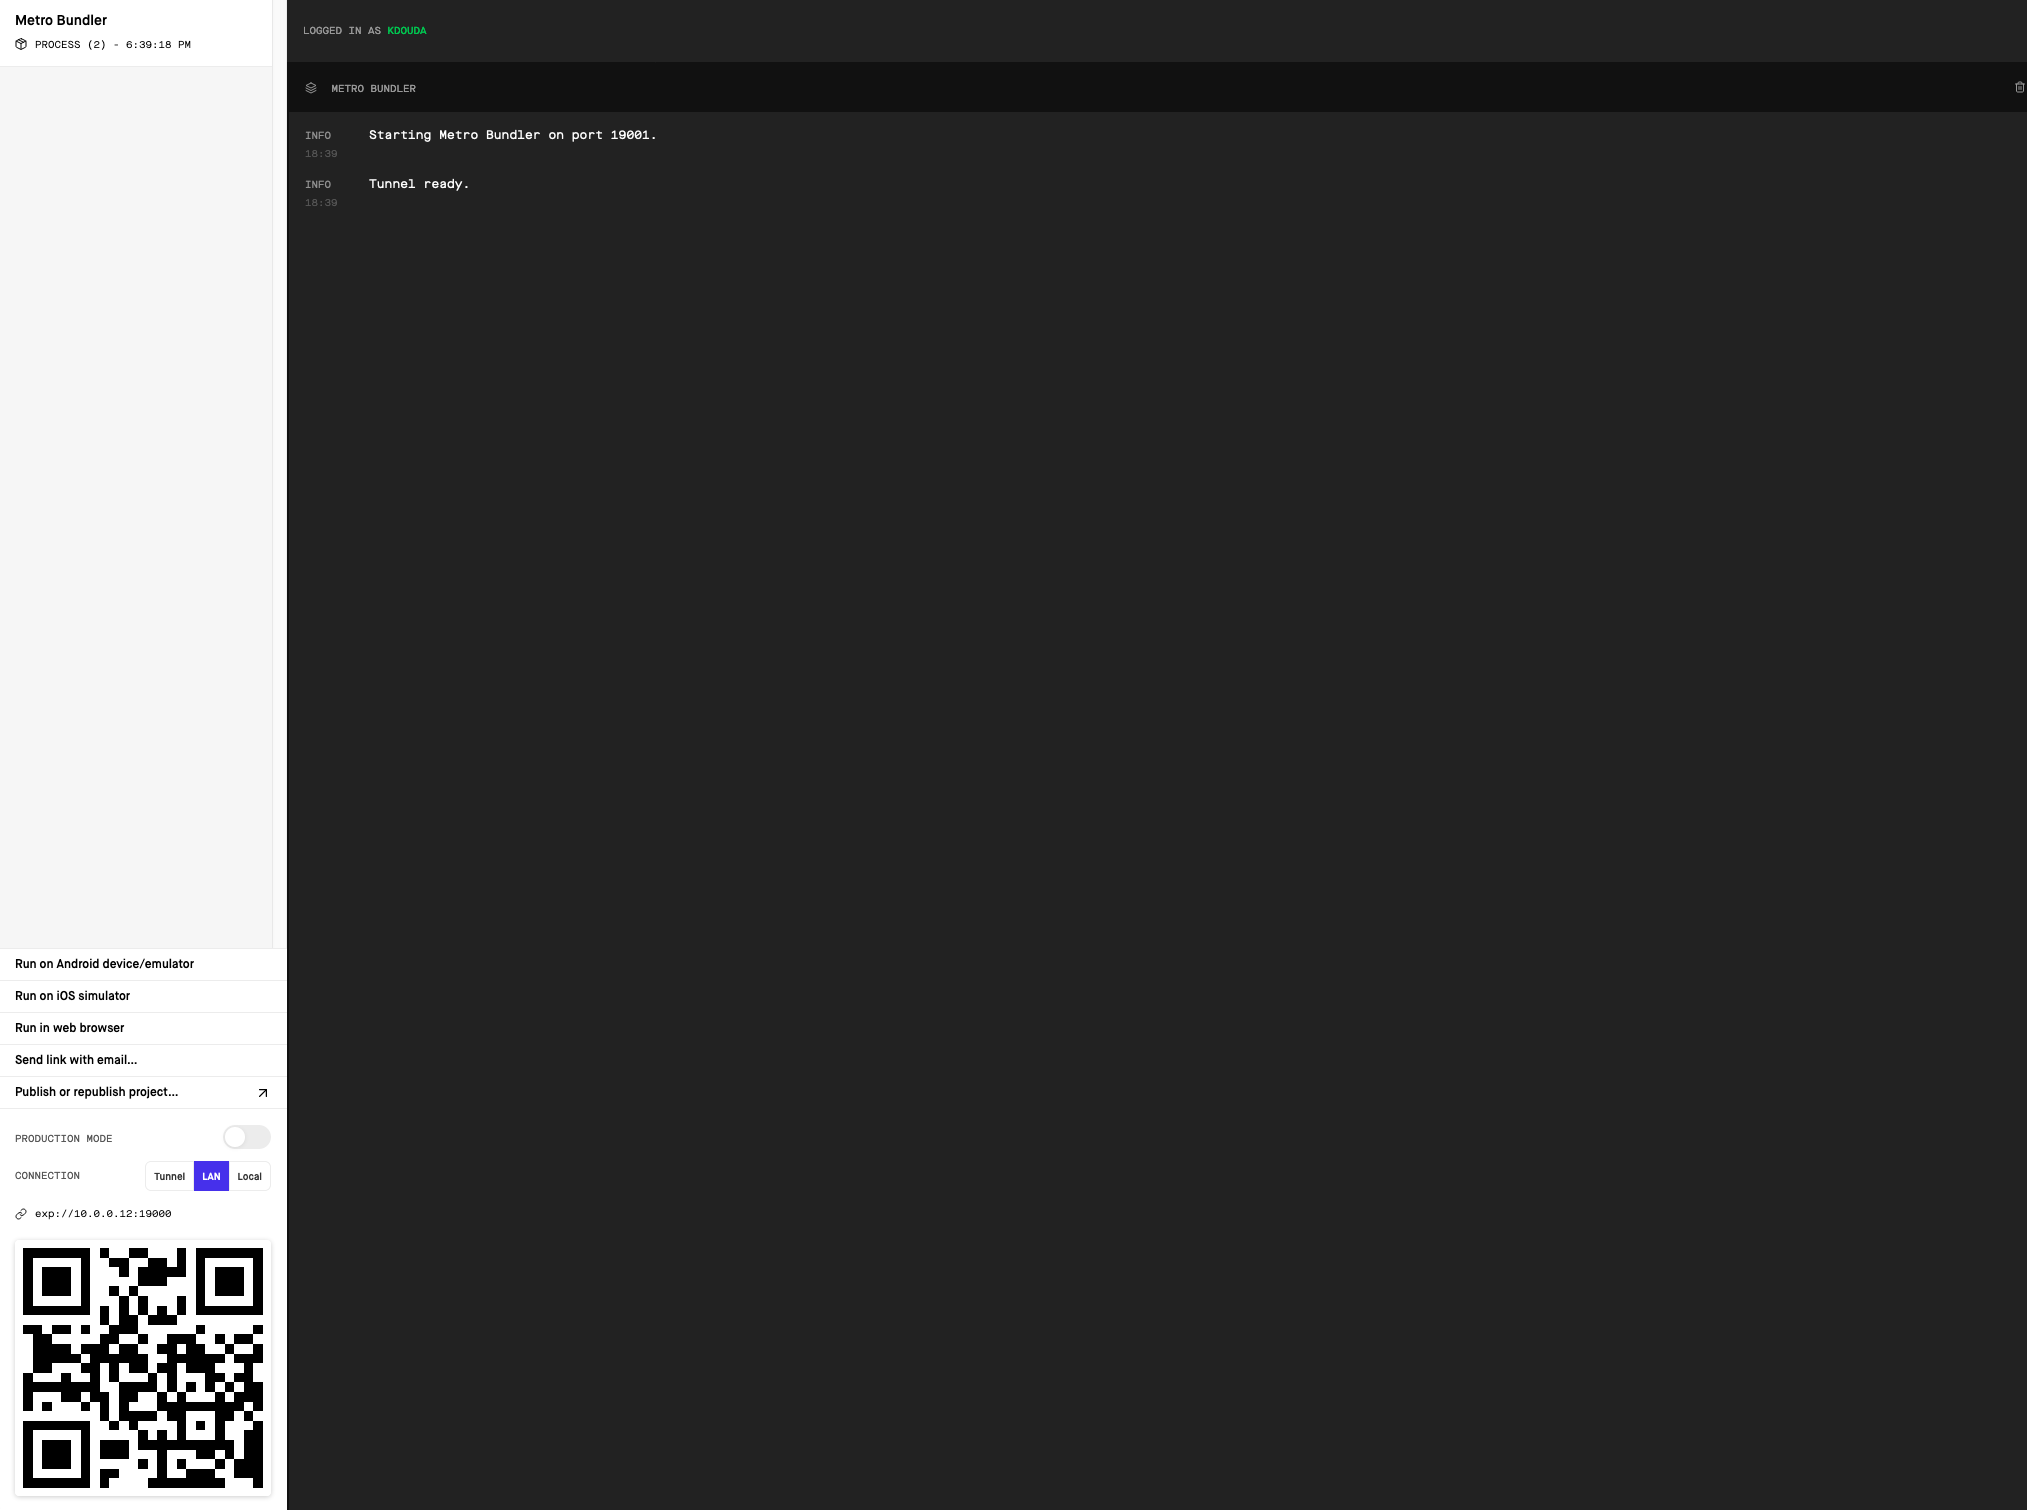
\includegraphics[width=140mm]{img/expo.png}
	\end{center}
	\caption{Expo -- zdroj: autor}
\end{figure}

\subsection{TurtleCLI}

TurtleCLI je nástroj pro sestavení Expo aplikací z příkazové řádky. Nástroj je určen pro uživatele, kteří si nepřejí využívat infrastruktury poskytované od Expo pro sestavování vlastních aplikací, ale přejí si aplikaci sestavit například na vlastním stroji nebo na vlastním nástroji kontinuální integrace.

Možnosti sestavení aplikací Expo jsou tedy dvojího typu, cloudové služby poskytované od Expo a TurtleCLI na vlastní infrastruktuře. Expo poskytuje cloudové služby zdarma ve variantě Community a placené prioritní zpracování ve variantě nazývané Priority.

Autor práce vybral tuto technologi z důvodu vysoké vytíženosti veřejné infrastruktury společnosti Expo (varianta nazývaná Community), kde jeho build ve frontě čekal v jednotkách hodin, než se dostal na řadu. Společnost Expo nabízí placenou variantu svých služeb, ve kterých avizuje výrazně vyšší rychlost odbavení, než u varianty zdarma a nástroje pro týmovou práci. Za značnou nevýhodu se taktéž může brát fakt, že kód je vždy odesílán třetí straně k sestavení, což pro mnoho firem může být nepřípustné. Oproti tomu provozování na vlastní infrastruktuře skýtá mnoho potenciálních výhod, za zmínku stojí napojení na firemní CI procesy, testovací infrastrukturu, rapidní nasazení mnoha paralelních větví do testovacích kanálů, jednodušší napojení sestavení na jiné akce. Níže je uvedena tabulka popisující podstatné rozdíly mezi jednotlivými způsoby sestavení Expo aplikací. 

\begin{table}[H]
	\begin{tabularx}{\textwidth}{|X|X|X|X|}
		\hline
		Kategorie                        & Community         & Priority      & Vlastní infrastruktura                 \\
		\hline
		Cena                             & zdarma            & 29 USD / měs. & cena výpočetního výkonu                \\
		\hline
		Čekací doba na začátek sestavení & cca. 1h           & minuty        & žádná                                  \\
		\hline
		Složitost zprovoznění            & součástí expo-cli & triviální     & dle zvolené varianty, nepříliš náročné \\
		\hline
		Provázanost s Expo               & vždy              & vždy          & žádná \\     
		\hline             
	\end{tabularx}
	\caption{Srovnání možností sestavení Expo aplikace}
\end{table}
%%% Fiktivní kapitola s ukázkami sazby

\chapter{Implementace}

Kapitola implementace se věnuje konkrétním akcím vedoucím k vytvoření spustitelného aplikačního artefaktu. V jednotlivých podkapitolách budou uvedeny využité prostředky, konkrétní kroky a jejich výstupy. Některé z těchto kroků jsou použitelné pro všechny Expo projekty a některé úsudky lze využít při vytváření vlastních Expo projektů. Za zmínku zde také stojí kapitola Implementace off-line map, ve které je popsán způsob jak zajistit funkční off-line mapy pro Expo projekty, pro co neexistují zatím žádné komunitní knihovny nebo Expo-nativní způsoby řešení.

\section{Vývojové prostředí}

% https://www.techopedia.com/definition/16376/development-environment

Vývojové prostředí je kolekce procedur a nástroj pro vývoj, testování a ladění aplikací nebo programů \cite{technopediaDevEnv}. Termín vývojové prostředí se používá v synonymu s termínem IDE, integrovaným vývojový prostředím, což je softwarový nástroj pro psaní, sestavení, testování a ladění programů. Do tohoto termínu taktéž lze zahrnout i nástroje co IDE samotné využívá pro setavení artefaktů.

Pro vývoj aplikace byly zvoleny následující nástroje vývojového prostředí:

\begin{itemize}
	\item VisualStudio Code jako nástroj IDE,
	\item Git jako verzovací nástroj,
	\item GitHub jako nástroj verzování i projektového řízení,
	\item AndroidStudio pro správu Android virtuálních strojů,
	\item XCode pro správu iOS virtuálních strojů (pouze na MacOS).
\end{itemize}

Dalším klíčovým softwarovým nástrojem je taktéž instalace Node.js a balíčkovacího nástroje NPM, bez kterých by byl vývoj Expo aplikace nemožný. Text této práce se jejich instalaci nevěnuje a předpokládá, že již nainstalované jsou. Instalace na běžných a aktuálních verzích OS není problémem.

Do pojmu vývojové prostředí se zahrnují i izolovaná prostředí, ve kterém běží testovací nebo produkční instance aplikace (resp. datového zdroje), v tomto případě platformy Anitra. Pro vývoj této aplikace nebylo toto rozlišení nutné a vyvíjelo se přímo na produkční verzi platformy Anitra.

\subsection{Vytvoření projektu}

V ukázce kódu \ref{expoinstall} bylo již zmíněno, jakým způsobem vytvořit Expo projekt. Pro vytvoření expo projektu stačí zadat následující příkazy do příkazové řádky.

\begin{lstlisting}[language=Bash, caption=Vytvoření nového projektu]
npm install --global expo-cli
expo init mobilni-aplikace
\end{lstlisting}

První řádek nainstaluje \emph{expo-cli}, nástroje pro vytváření, správu, spouštění a sestavení Expo projektů. Druhý příkaz vytvoří nový expo projekt \emph{mobilni-aplikace} v aktuální složce uživatele.

Z předpřipraveného kódu je dobré zmínit vstupní bod aplikace \emph{App.tsx}, ve kterém je připravená ukázková komponenta. Z tohoto vstupního bodu se implementují navigátory zmíněné v kapitole Implementace navigátorů.

\section{Implementace úložišť a entit}

Implementace úložišť a entit byla vytvořena dle návrhu aplikace. Bylo vytvořeno více entit, než bylo plánováno, aby celá aplikace komunikovala za pomocí typovaných objektů a tím se zjednodušil proces ladění v aplikaci i urychlil vývoj. Pro entity bylo využito rozhraní, aby entity pro funkce ukládání měly stejnou signaturu a bylo je možné používat ve stylu OOP bez složitých konstrukcí. V ukázce kódu uvedené níže je ukázáno rozhraní, které musí implementovat všechny entity a entity, které mají být uložitelné na disk.

\begin{lstlisting}[language=JavaScript, caption=Ukázka entity]
export interface IEntity {
	id?: number;
	
	synchronized: boolean;
	lastSynchronized?: Date;
};

export interface ISerializableEntity extends IEntity {
	toJson() : object;
	
	toJsonString() : string;
	
	fromJson(json: any): IEntity;
};
\end{lstlisting}

Implementace úložišť samotných spočívá v implementaci tří částí -- v komunikaci se serverem, transformaci dat od serveru a uložení těchto dat na disk. Pro komunikaci se serverem pomocí HTTP Rest API byla zvolena knihovna \emph{axios}, která se běžně používá v JavaScriptových projektech pro abstrakci rozdílů mezi jednotlivými klienty. Knihovna dále umožňuje jednodušší přístup např. k hlavičkám HTTP dotazu a je tedy jednoduché se např. oproti vzdálenému serveru autentifikovat. Axios očekává na vstupu objekt obsahující výčet parametrů a na výstupu vrací tělo dotazu zformátované do správného formátu (např. když server vrací JSON odpověď, Axios z vráceného textu správně složí JSON).

Transformace dat ze serveru spočívá v převodu klíčů a hodnot vrácených ze serveru do předem zmíněných entit. Entity v aplikaci neobsahují celá data, ale pouze výčet, který aplikace skutečně potřebuje. Tímto se šetří nejen místo na disku, ale i doba serializace a deserializace entit při čtení z disku. V API nejde stanovit, jaká pole dotazovatel vyžaduje a filtrování je tedy nutno provést až na koncovém bodu procesu, tedy v mobilní aplikaci.

Pro uložení dat byla využita součást Expo \emph{expo-file-system}, která abstrahuje od jednotlivých souborových systémů operačních systémů. Nevýhodou tohoto systému je neobratnost při zakládání složek, složky se musí vytvářet dopředu a nelze je vytvořit při zápisu souboru. Podstatnější nevýhodou je nutnost serializovat obsah souboru do textu, a nejedná se tedy o příliš vhodnou metodu ukládání např. obrazových dat kvůli nutnosti převést binární data na textový formát např. Base64. Alternativní řešení pro Expo neexistuje. Ukázka práce se souborovým systémem je v následující ukázce kódu.

\begin{lstlisting}[language=JavaScript, caption=Ukázka entity]
import * as FileSystem from 'expo-file-system';

let string = await FileSystem.readAsStringAsync(path);
\end{lstlisting}

Do proměnné string se asynchronně zapíše obsah souboru v cestě, v případě chyby čtení, např. způsobené neexistujícím souborem, se vyhodí výjimka. Soubor lze dále zpracovat předevím např. textu na JSON nebo na XML, případně jakýkoliv jiný formát, který aplikace využívá. V aplikaci se nad těmito funkcemi staví třída PersistenStorage, která poskytuje obecné metody pro uložení a získání kolekcí či jednotlivých entit.

\section{Implementace obrazovek}

Implementace obrazovek byla nejdelší částí tvorby aplikace a nejnáročnější na testování. Obrazovky jsou React komponenty umístěny ihned pod navigátorem. V jejich životním cyklu se vytváří subkomponenty, získávají data z úložišť a pomocí událostí komunikují s úložišti. Obrazovky jsou spolu se subkomponentami zodpovědné za správu interakcí s uživatelem.

Níže je uvedena ukázková implementace obrazovky AuthLoading, která rozhoduje o přesměrování uživatele po zapnutí aplikace, pokud je přihlášen či ne.

\begin{lstlisting}[language=JavaScript, caption=Ukázka implementace obrazovky]
import React from 'react';
import { StyleSheet, Text, View } from 'react-native';
import { MaterialIndicator } from 'react-native-indicators';

import AuthStore from '../store/AuthStore';
import Theme from "../constants/Theme.js";

export default class AuthLoading extends React.Component {
	verifyAuth = async () => {
		await AuthStore.awaitAuth();
		if (AuthStore.isAuthorized) {
			this.props.navigation.navigate("Map");
		} else {
			this.props.navigation.navigate("AuthContainer");
		}
	}
	
	componentDidMount() {
		this.verifyAuth();
	}
	
	render () {
		return (
		<View style={styles.container}>
			<View>
				<MaterialIndicator color={ Theme.colors.brand.primary }/>
			</View>
		</View>
		);
	}
}

const styles = StyleSheet.create({
	container: {
		flex: 1,
		backgroundColor: Theme.colors.default.background,
		alignItems: 'center',
		justifyContent: 'center',
		alignSelf: 'stretch',
	}
});

\end{lstlisting}

V ukázce lze vidět několik podstatných částí. V první části jsou importy závislostí, kde veškeré obrazovky potřebují naimportovat alespoň závislost \emph{React} z knihovny React. Na druhém řádku lze vidět import typických ovládacích prvků a utilit pro obrazovku či subkomponentu. StyleSheet je způsob zapsání stylu pro ReactNative, ukázka způsobu zápisu stylů se nachází v objektu \emph{styles} na konci ukázky kódu. Text je komponenta, která umožňuje zobrazení stylovaného textu a jako jediná může obsahovat čistý text. Komponenta View rámcově odpovídá funkci tagu \emph{div} v HTML a je pouze prázdným kontejnerem pro ostatní komponenty, ale může být stylována. Následně je vidět import \emph{MaterialIndicator} z knihovny \emph{react-native-indicators}, externí komponenty, která zobrazuje načítací spinner, aby UI nevypadala neresponzivně. Následně je importováno úložiště pro autentifikaci a seznam konstant obsahující styl aplikace.

Samotná obrazovka začíná na řádku 8, kde se nachází definice třídy komponenty. Na řádku devět se nachází metoda komponenty, ve které se volá úložiště Auth pro ověření, zda je uživatel autorizovaný, a případně se přenaviguje na správnou obrazovku. Vysoce podstatná je metoda \emph{componentDidMount} na řádku 18, která se spustí po načtení komponenty a volá již zmiňovanou funkci na ověření přihlášení. Metoda render vrací JSX obrazovky, tedy strukturu všech subkomponent. Na konci je již zmiňovaný objekt styles, obsahující styly.

Tato obrazovka je reprezentativní pro všechny obrazovky, s výjimkou hlavní mapy.

\subsection{Implementace hlavní mapy}

Pro hlavní část této obrazovky, tedy mapy, byla využita knihovna \emph{react-native-maps} z důvodu absence alternativ pro Expo. Knihovna však splňuje veškeré požadavky aplikace. Do mapy lze např. vkládat objekty typu trasa, bod i tyto body následně stylovat. Objekty do mapy se přidávají jako individuální komponenty, např. bod s tzv. infoboxem (bublinou nad bodem) se vytvoří následujícím způsobem.

\begin{lstlisting}[language=JavaScript, caption=Ukázka implementace obrazovky]
<MapView>
	<Marker
		coordinate={ { latitude: point.lat, longitude: point.lng } }
		icon={image}
		image={image}
		zIndex={zIndex}
	>
		<Callout>
			<MarkerPosition tracking={track.tracking} id={point.id}/>
		</Callout>
	</Marker>
</MapView>
\end{lstlisting}

Ukázka ilustruje způsob umístění v mapě (parametr coordinate), způsob vybrání ikony pro obě platformy (parametr icon a image) a nastavení zIndexu, který určuje pořadí vykreslování komponent vzájemně se překrývajících. Komponenta Callout obsahuje již zmiňované infowindow, které obsahuje subkomponentu MarkerPosition.

Pro implementaci vyjížděcího menu pro filtry byla využita komponenta \emph{rn-sliding-up-panel}, která plně splina zadání z kapitoly návrh. Detaily implementace lze zobrazit v příloze, jelikož jsou příliš dlouhé pro ukázky v textu této práce.

\begin{figure}[H]
	\begin{center}
		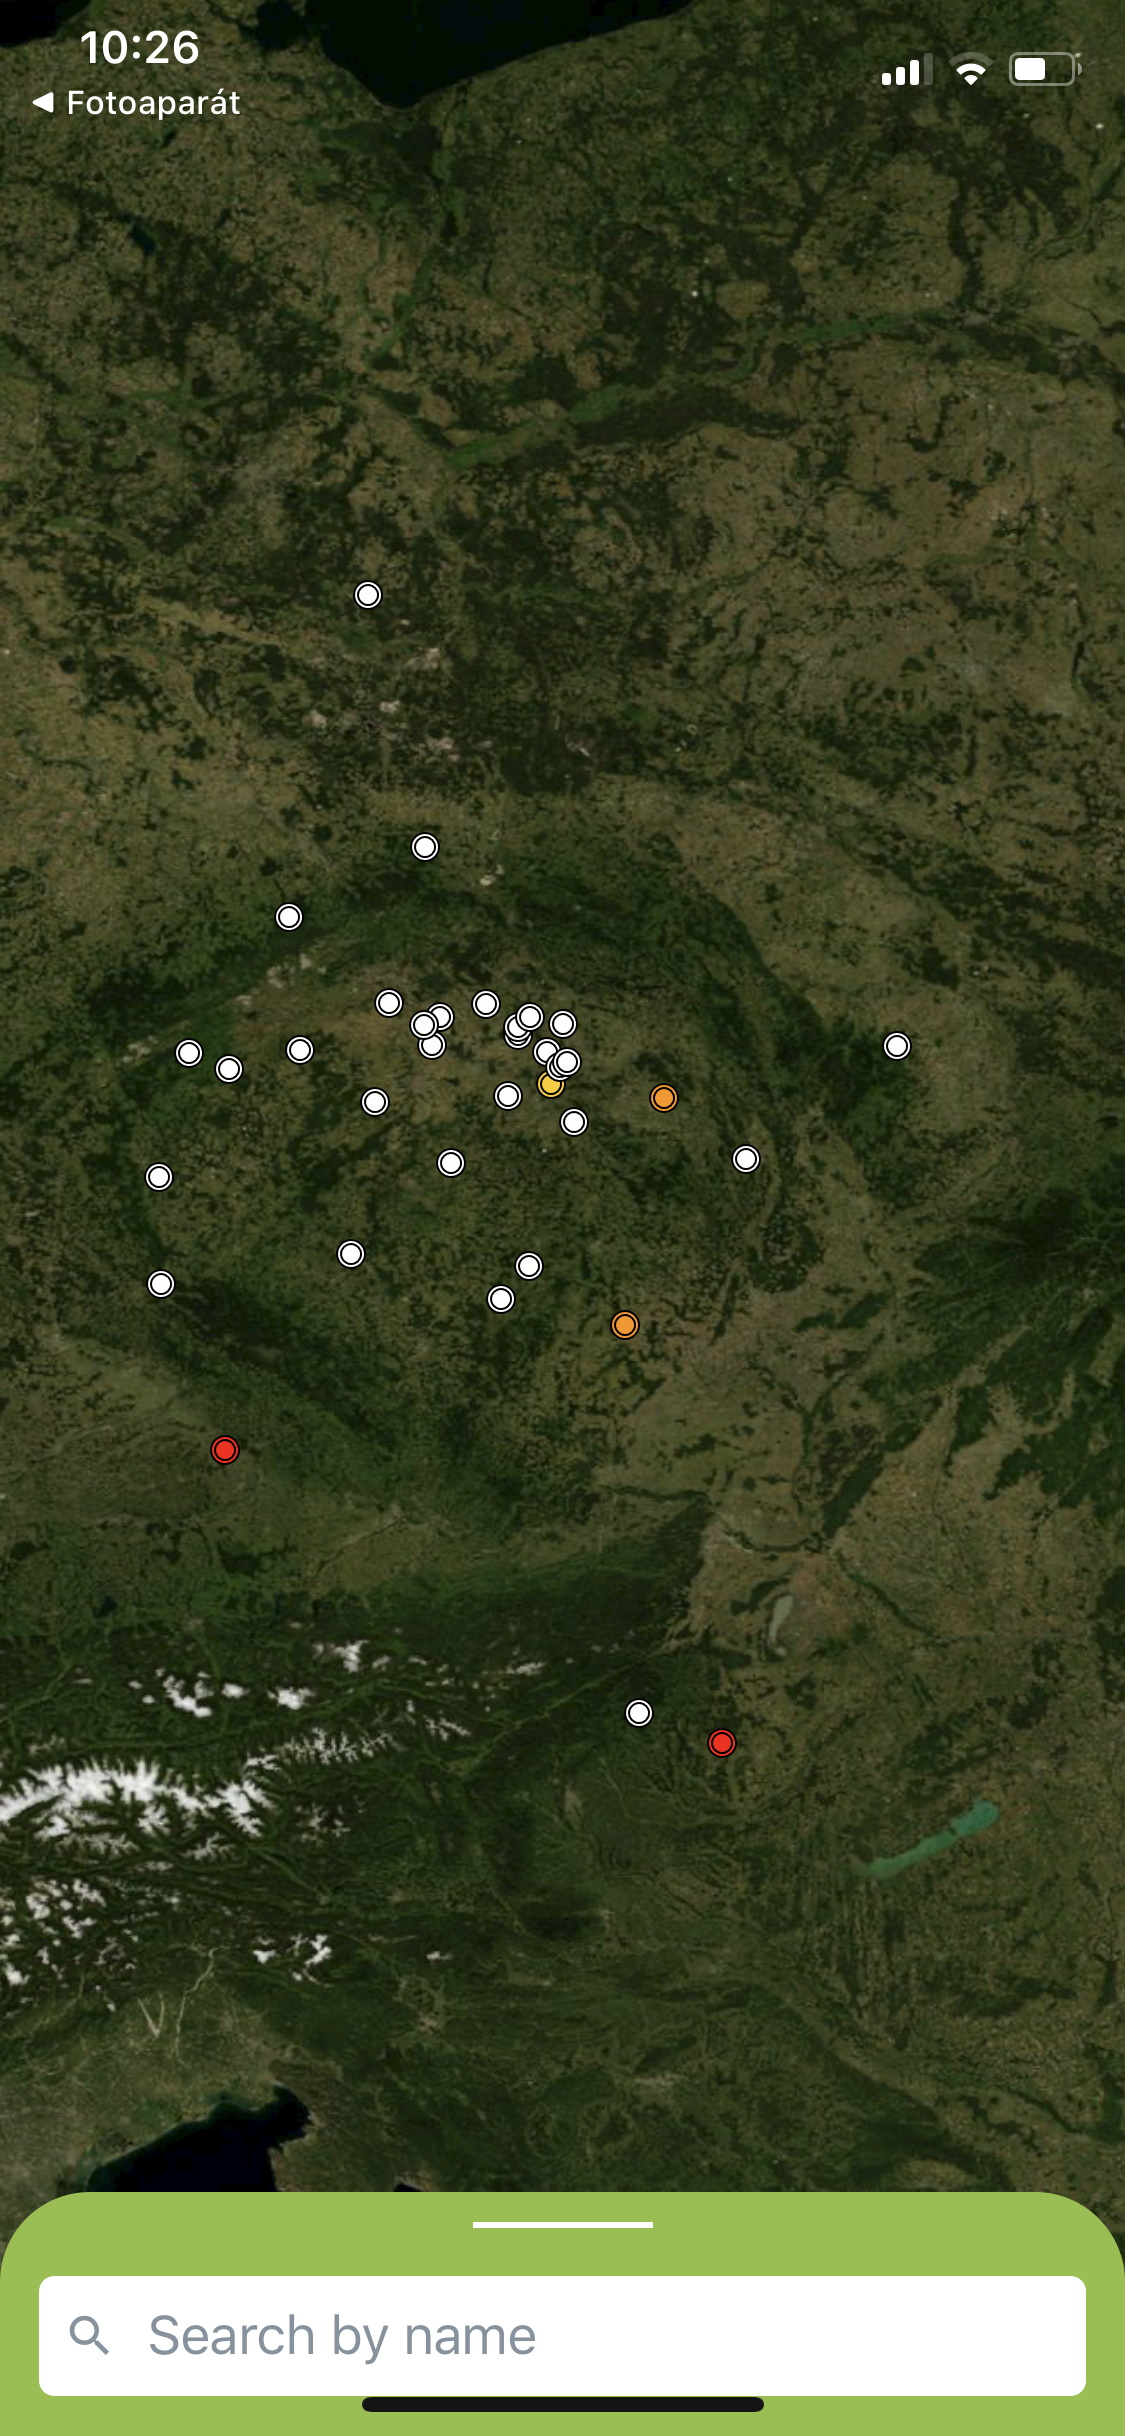
\includegraphics[width=70mm]{img/example_map.jpg}
	\end{center}
	\caption[Výsledek implementace hlavní mapy]{Výsledek implementace hlavní mapy -- zdroj: autor}
\end{figure}

Výsledek implementace mapy je srovnatelný s drátěným modelem představeným v kapitole Návrh.

\section{Implementace subkomponent}

Subkomponenty byly vytvořeny pro splnění mapové koncepce, tedy pro jednotlivé overlay funkce definované v kapitole návrh. Zbylé subkomponenty byly vytvářeny dle potřeby pro zpřehlednění aplikace, tedy ad hoc. Za zvláštní zmínku stojí implementace off-line map, která byla vytvořena čistě pro tuto aplikaci.

\subsection{Implementace off-line map}

Pro implementace off-line map bylo nutno vytvořit dvě komponenty. První komponentou jsou off-line mapy samotné, druhou komponentou způsob, jak vybrat rozsah, který má být stažen.

Off-line schopnost map je umožněna díky následujícím klíčovým možnostem: možnost načítat tzv. tile mapy (mapy uložené ve formátu obrázků s jednoznačným indexem v dimenzích x, y a z) a URI, které využívá Expo i pro ukládání souborů. Pro mapy je tedy jedno, zda načítají jednotlivé mapové čtverečky z disku, či přímo ze vzdáleného mapového serveru.

\begin{lstlisting}[language=JavaScript, caption=Off-line mapy]
import { UrlTile } from 'react-native-maps';
<MapView..>
	<UrlTile urlTemplate="..."/>
</MapView>
\end{lstlisting}

Do urlTemplate se místo vzdáleného zdroje doplní část kódu, která obsahuje parametry pro jednotlivé dimenze mapy ve formátu \emph{\{z\}/\{x\}/\{y\}.png}. Každý mapový čtvereček je následně načítán z disku. Toto chování je vhodné zapnout pouze v případě že uživatel není připojený k síti, či na přímé vyžádání uživatele.

Kvůli nedostatku času nebylo možné vytvořit komfortní uživatelský nástroj pro výběr off-line map, a vznikl proto pouze rudimentární. Z kontextového menu uživatel zapne dialog zadávání bodů, čímž se uloží příznak do aplikace, že uživatel vybírá off-line region. Uživatel je následně instruován, aby klikal do mapy.

\section{Implementace navigátorů}

Pro implementaci navigátorů byla vybrána již zmiňovaná standardní knihovna \emph{react-navigation}. Pro instalaci je využitý balíčkovací nástroj NPM.

\begin{lstlisting}[language=Bash, caption=Instalace react-navigation]
npm install react-navigation
npm install react-navigation-stack
\end{lstlisting}

Po instalaci je nejprve ve vybrané React komponentě nejprve naimportovat dané knihovny. 

\begin{lstlisting}[language=JavaScript, caption=Import knihoven pro hlavní navigátor]
import { createSwitchNavigator, createAppContainer, NavigationContainerComponent, NavigationActions } from 'react-navigation';
import { createStackNavigator } from 'react-navigation-stack';
\end{lstlisting}

Importováním těchto závislostí půjde vytvořit switch navigátor, hlavní navigační kontejner aplikace a stack navigátor. Následně je nutné naimportovat komponenty obrazovek následujícím způsobem.

\begin{lstlisting}[language=JavaScript, caption=Import obrazovek pro hlavní navigátor]
import Welcome from './src/screens/auth/Welcome'; // naimportuje komponentu obrazovky Welcome
import Login from './src/screens/auth/Login';
import Register from './src/screens/auth/Register';
import MapScreen from './src/screens/in/Map';
\end{lstlisting}

Navigátory lze následně sestavit modulárním způsobem vkládání do sebe, kde listy grafu navigátorů jsou jednotlivé komponenty obrazovek.

\begin{lstlisting}[language=JavaScript, caption=Implementace navigátorů]
const AuthContainer = createStackNavigator({
	Welcome: Welcome,
	Login: Login,
	Register: Register
}, {
	headerMode: 'none'
});

const AppNavigator = createSwitchNavigator({
	AuthLoading: AuthLoading,
	Map: MapScreen,
	AuthContainer: AuthContainer
}, {
	"initialRouteName": "AuthLoading" // nazev vychozi cesty, resp. obrazovkove komponenty
});
\end{lstlisting}

Navigátory se následně obalí aplikačním kontejnerem, ze kterého se vytvoří hlavní komponenta aplikace, tedy její vstupní bod.

\begin{lstlisting}[language=JavaScript, caption=Vytvoření aplikačního kontejneru]
const AppContainer = createAppContainer(
	AppNavigator
);

export default class App extends React.Component
{
	render () {
		return (
				<React.Fragment>
					<AppContainer ref = { setNavigatorRef }/>
					<FlashMessage position="top" />
				</React.Fragment>
		)
	}
}
\end{lstlisting}

V ukázce kódu se vytváří komponenta App, která je vstupním bodem aplikace. V komponentě App se nachází fragment, který je kolekcí různých React komponent a sám nemá v uživatelském rozhraní žádnou funkci. Následně se vytvořený AppContainer využije přímo v komponentě a jeho vykresleným obsahem se stávají různé obrazovky specifikované v předchozích ukázkách kódu. Ačkoliv se nejedná přímo o funkce navigátoru, na stejné úrovni se také nachází komponenta FlashMessage, která zajistí, že se tzv. flash zprávy vygenerované v aplikaci zobrazují napříč všemi obrazovkami z jednoho místa (tedy bez duplikace kódu). Nejedná se tedy o funkci navigátoru, ale pouze o komponentu, kterou je vhodné umístit na nejvyšší úroveň kvůli prevenci duplikaci kódu a jedná se o vhodnou ukázku, co lze na stejnou úroveň jako kontejner navigátorů vložit.

Pro přenavigování lze využít v jakékoliv komponentě umístěné pod AppContainerem (resp. pod jakýmkoliv navigátorem) funkcí uvedenou níže.

\begin{lstlisting}[language=JavaScript, caption=Přenavigování]
this.props.navigation.navigate("Map");
\end{lstlisting}

Všem komponentám je předán odkaz na navigátor a pomocí klíče (názvu) obrazovky se na ni lze přenavigovat kdekoliv uvnitř komponenty, např. při reagování na kliknutí z tlačítka či doběhnutím vnitřní události. Navigace mimo komponentu ale tímto způsobem není možná, proto byl autorem aplikace v App.tsx vytvořena možnost, jak tuto funkci z komponenty získat. V komponentě AppContainer byl specifikován atribut ref. Atribut ref v Reactu slouží k získání instance určité komponenty. Komponenta se předá funkci setNavigatorRef, který do lokální proměnné vloží instanci navigátoru. Aplikace nad touto lokální instancí vytváří funkci navigate, ve které volá událost navigace a je tedy možné z kódu mimo komponenty volat funkce navigace.

\begin{lstlisting}[language=JavaScript, caption=Přenavigování]
let instanceRef: NavigationContainerComponent;

function setNavigatorRef(instance: NavigationContainerComponent) {
	instanceRef = instance;
}

function navigate(routeName, params) {
	instanceRef.dispatch(
		NavigationActions.navigate({
			routeName,
			params,
		})
	);
}
\end{lstlisting}

\section{Implementace push notifikací}

Jednou z mnoha výhod platformy Expo je jednoduchost napojení aplikačních push notifikací. Není potřeba využívat různé poskytovatele pro různé platformy, Expo zajistí doručení na jakékoliv zařízení, které se k notifikacím registruje. Výhodou také je jednoduchost celého systému, kde stačí aby se zařízení pouze oznámilo serveru svým identifikátorem a následně lze notifikace volat za pomocí REST API Expo. Celý proces je velmi jednoduchý na implementaci v mobilní aplikaci i ve zdroji notifikací. Získání notifikací na straně aplikace lze docílit následujícím způsobem.

\begin{lstlisting}[language=JavaScript, caption=Expo notifikace]
import { Notifications } from 'expo';
import * as Permissions from 'expo-permissions';
import Constants from 'expo-constants';


const { status } = await Permissions.askAsync(Permissions.NOTIFICATIONS);

if (finalStatus !== 'granted') {
	return;
}

const token = await Notifications.getExpoPushTokenAsync();
\end{lstlisting}

Pro notifikace je třeba získat svolení uživatele. Pokud svolení dá, Expo vrátí textový token, který se následně dá použít k poslání notifikace na konkrétní zařízení. Pro zjednodušení práce s větším počtem stejných notifikací je možnost vytvářet skupiny příjemců, aplikace ji nevyužívá. Kód pro generování zpráv na straně serveru není součástí této práce a je pouze obsažen ve webovém backendu aplikace Anitra.

% \section{Sestavení pomocí TurtleCLI}

% \section{Publikování na Google Play}
\chapter*{Závěr}
\addcontentsline{toc}{chapter}{Závěr}

Cílem této práce bylo vytvořit offline-capable mobilní aplikaci splňující požadavky ornitologů pro práci v poli. Tento cíl byl splněn vytvořením aplikace ve frameworku React Native, resp. Expo. Aplikace byla vytvořena a otestována autorem na obou hlavních mobilních platformách. Aplikace kvůli komplikacím způsobené COVID-19 nemohla být včas nasazena, jelikož distribuční platformy nestíhaly zpracovávat požadavky na nové aplikace, nebylo ani možné distribuovat testovací verzi vybrané sekci potenciálních uživatelů. 

Vývoj aplikace bude pokračovat a stane se užitečnou pomůckou při výzkumných projektech klientů platformy Anitra. Ostrý provoz aplikace se očekává po červnu 2020, kdy se do aplikace doimplementují některé chybějící moduly a aplikace se výrazně zoptimalizuje. Klientům bude dodána přes internetové obchody mobilních aplikací Android Google Play a iOS App Store, o vydání aplikace se dozví z newsletteru platformy Anitra či z webové stránky. 

%%% Seznam použité literatury
%% Toto platí v případě použití samostatné bibliografické databáze
\printbibliography[title={Seznam použité literatury},heading={bibintoc}]

%% Toto platí v případě použití prostředí thebibliography
%% Pro sestavení citačních údajů lze doporučit:
%%     https://knihovna.vse.cz/citace/priklady/
%%     https://www.citace.com/
%\openright
%\phantomsection
%\addcontentsline{toc}{chapter}{\bibname}
%\begin{thebibliography}{99}
%\bibitem{Cermak2018}ČERMÁK, Radim, SMUTNÝ, Zdeněk. A Framework for Cultural Localization of Websites and for Improving Their Commercial Utilization. In:  \emph{Global Observations of the Influence of Culture on Consumer Buying Behavior} [online]. Hershey~: IGI Global, 2018, s. 206--232. ISBN 978-1-5225-2727-5. DOI: 10.4018/978-1-5225-2727-5.
%
%\bibitem{Hladik2018}HLADÍK, Milan, ČERNÝ, Michal. The Shape of the Optimal Value of a Fuzzy Linear Programming Problem. In: \emph{Fuzzy Logic in Intelligent System Design} [online]. Cancum, 16.10.2017 -- 18.10.2017. Cham~: Springer, 2018, s. 281--286. Advances in Intelligent Systems and Computing 648. ISBN 978-3-319-67136-9. DOI: 10.1007/978-3-319-67137-6\_31.
%
%\bibitem{Jasek2018}JAŠEK, Pavel, VRANÁ, Lenka, ŠPERKOVÁ, Lucie, SMUTNÝ, Zdeněk, KOBULSKÝ, Marek. Modeling and Application of Customer Lifetime Value in Online Retail. \emph{Informatics} [online]. 2018, roč. 5, č. 1. 22 s. eISSN 2227-9709. DOI: 10.3390/informatics5010002. Dostupné také z: \url{http://www.mdpi.com/2227-9709/5/1/2/pdf}.
%
%\bibitem{Pecakova2018}PECÁKOVÁ, Iva. \emph{Statistika v terénních průzkumech}. 3. přeprac. vyd. Praha~: Professional Publishing, 2018. 254 s. ISBN 978-80-88260-10-3.
%\end{thebibliography}


%%% Přílohy k bakalářské práci, existují-li. Každá příloha musí být alespoň jednou
%%% odkazována z vlastního textu práce. Přílohy se číslují.
\part*{Přílohy}
\appendix
\chapter{Formulář v plném znění}

\chapter{Zdrojové kódy výpočetních procedur}


% \include{...}
% \include{...}

\end{document}
